%%%%%%%%%%%%%%%%%%%%%%%%%%%%%%%%%%%%%%%%%%%%%%%%%%%%%%%%%%%%%%%%%%%%%%
% Template for a UBC-compliant dissertation
% At the minimum, you will need to change the information found
% after the "Document meta-data"
%
%!TEX TS-program = pdflatex
%!TEX encoding = UTF-8 Unicode

%% The ubcdiss class provides several options:
%%   gpscopy (aka fogscopy)
%%       set parameters to exactly how GPS specifies
%%         * single-sided
%%         * page-numbering starts from title page
%%         * the lists of figures and tables have each entry prefixed
%%           with 'Figure' or 'Table'
%%       This can be tested by `\ifgpscopy ... \else ... \fi'
%%   10pt, 11pt, 12pt
%%       set default font size
%%   oneside, twoside
%%       whether to format for single-sided or double-sided printing
%%   balanced
%%       when double-sided, ensure page content is centred
%%       rather than slightly offset (the default)
%%   singlespacing, onehalfspacing, doublespacing
%%       set default inter-line text spacing; the ubcdiss class
%%       provides \textspacing to revert to this configured spacing
%%   draft
%%       disable more intensive processing, such as including
%%       graphics, etc.
%%

% For submission to GPS
\documentclass[gpscopy,onehalfspacing,11pt]{ubcdiss}

% For your own copies (looks nicer)
% \documentclass[balanced,twoside,11pt]{ubcdiss}

%%%%%%%%%%%%%%%%%%%%%%%%%%%%%%%%%%%%%%%%%%%%%%%%%%%%%%%%%%%%%%%%%%%%%%
%%%%%%%%%%%%%%%%%%%%%%%%%%%%%%%%%%%%%%%%%%%%%%%%%%%%%%%%%%%%%%%%%%%%%%
%%
%% FONTS:
%% 
%% The defaults below configures Times Roman for the serif font,
%% Helvetica for the sans serif font, and Courier for the
%% typewriter-style font.  Configuring fonts can be time
%% consuming; we recommend skipping to END FONTS!
%% 
%% If you're feeling brave, have lots of time, and wish to use one
%% your platform's native fonts, see the commented out bits below for
%% XeTeX/XeLaTeX.  This is not for the faint at heart. 
%% (And shouldn't you be writing? :-)
%%

%% NFSS font specification (New Font Selection Scheme)
\usepackage{times,mathptmx,courier}
\usepackage[scaled=.92]{helvet}

%% Math or theory people may want to include the handy AMS macros
%\usepackage{amssymb}
%\usepackage{amsmath}
%\usepackage{amsfonts}

%% The pifont package provides access to the elements in the dingbat font.   
%% Use \ding{##} for a particular dingbat (see p7 of psnfss2e.pdf)
%%   Useful:
%%     51,52 different forms of a checkmark
%%     54,55,56 different forms of a cross (saltyre)
%%     172-181 are 1-10 in open circle (serif)
%%     182-191 are 1-10 black circle (serif)
%%     192-201 are 1-10 in open circle (sans serif)
%%     202-211 are 1-10 in black circle (sans serif)
%% \begin{dinglist}{##}\item... or dingautolist (which auto-increments)
%% to create a bullet list with the provided character.
\usepackage{pifont}

%%%%%%%%%%%%%%%%%%%%%%%%%%%%%%%%%%%%%%%%%%%%%%%%%%%%%%%%%%%%%%%%%%%%%%
%% Configure fonts for XeTeX / XeLaTeX using the fontspec package.
%% Be sure to check out the fontspec documentation.
%\usepackage{fontspec,xltxtra,xunicode}	% required
%\defaultfontfeatures{Mapping=tex-text}	% recommended
%% Minion Pro and Myriad Pro are shipped with some versions of
%% Adobe Reader.  Adobe representatives have commented that these
%% fonts can be used outside of Adobe Reader.
%\setromanfont[Numbers=OldStyle]{Minion Pro}
%\setsansfont[Numbers=OldStyle,Scale=MatchLowercase]{Myriad Pro}
%\setmonofont[Scale=MatchLowercase]{Andale Mono}

%% Other alternatives:
%\setromanfont[Mapping=tex-text]{Adobe Caslon}
%\setsansfont[Scale=MatchLowercase]{Gill Sans}
%\setsansfont[Scale=MatchLowercase,Mapping=tex-text]{Futura}
%\setmonofont[Scale=MatchLowercase]{Andale Mono}
%\newfontfamily{\SYM}[Scale=0.9]{Zapf Dingbats}
%% END FONTS
%%%%%%%%%%%%%%%%%%%%%%%%%%%%%%%%%%%%%%%%%%%%%%%%%%%%%%%%%%%%%%%%%%%%%%
%%%%%%%%%%%%%%%%%%%%%%%%%%%%%%%%%%%%%%%%%%%%%%%%%%%%%%%%%%%%%%%%%%%%%%



%%%%%%%%%%%%%%%%%%%%%%%%%%%%%%%%%%%%%%%%%%%%%%%%%%%%%%%%%%%%%%%%%%%%%%
%%%%%%%%%%%%%%%%%%%%%%%%%%%%%%%%%%%%%%%%%%%%%%%%%%%%%%%%%%%%%%%%%%%%%%
%%
%% Recommended packages
%%
\usepackage{checkend}	% better error messages on left-open environments
\usepackage{graphicx}	% for incorporating external images
\usepackage{tikz}
\usepackage{amsmath}

% inlined bib file
\usepackage{filecontents}

\usepackage[utf8]{inputenc}%(only for the pdftex engine)
\usepackage{amsmath}
\usepackage{graphicx}
\usepackage{subcaption}
\usepackage{indentfirst}
\usepackage{listings}
\usepackage{color, colortbl}
\usepackage{xcolor}
\usepackage{multirow}
\usepackage{url}%[hyphens]
\usepackage{enumitem}
\usepackage{bbding}
\usepackage{diagbox}
%% booktabs: provides some special commands for typesetting tables as used
%% in excellent journals.  Ignore the examples in the Lamport book!
\usepackage{booktabs}

%% listings: useful support for including source code listings, with
%% optional special keyword formatting.  The \lstset{} causes
%% the text to be typeset in a smaller sans serif font, with
%% proportional spacing.
\usepackage{listings}
\lstset{basicstyle=\sffamily\scriptsize,showstringspaces=false,fontadjust}

%% The acronym package provides support for defining acronyms, providing
%% their expansion when first used, and building glossaries.  See the
%% example in glossary.tex and the example usage throughout the example
%% document.
%% NOTE: to use \MakeTextLowercase in the \acsfont command below,
%%   we *must* use the `nohyperlinks' option -- it causes errors with
%%   hyperref otherwise.  See Section 5.2 in the ``LaTeX 2e for Class
%%   and Package Writers Guide'' (clsguide.pdf) for details.
\usepackage[printonlyused,nohyperlinks]{acronym}
%% The ubcdiss.cls loads the `textcase' package which provides commands
%% for upper-casing and lower-casing text.  The following causes
%% the acronym package to typeset acronyms in small-caps
%% as recommended by Bringhurst.
\renewcommand{\acsfont}[1]{{\scshape \MakeTextLowercase{#1}}}

%% color: add support for expressing colour models.  Grey can be used
%% to great effect to emphasize other parts of a graphic or text.
%% For an excellent set of examples, see Tufte's "Visual Display of
%% Quantitative Information" or "Envisioning Information".
\usepackage{color}
\definecolor{greytext}{gray}{0.5}

%% comment: provides a new {comment} environment: all text inside the
%% environment is ignored.
%%   \begin{comment} ignored text ... \end{comment}
\usepackage{comment}

%% The natbib package provides more sophisticated citing commands
%% such as \citeauthor{} to provide the author names of a work,
%% \citet{} to produce an author-and-reference citation,
%% \citep{} to produce a parenthetical citation.
%% We use \citeeg{} to provide examples
\usepackage[numbers,sort&compress]{natbib}
\newcommand{\citeeg}[1]{\citep[e.g.,][]{#1}}

%% The titlesec package provides commands to vary how chapter and
%% section titles are typeset.  The following uses more compact
%% spacings above and below the title.  The titleformat that follow
%% ensure chapter/section titles are set in singlespace.
\usepackage[compact]{titlesec}
\titleformat*{\section}{\singlespacing\raggedright\bfseries\Large}
\titleformat*{\subsection}{\singlespacing\raggedright\bfseries\large}
\titleformat*{\subsubsection}{\singlespacing\raggedright\bfseries}
\titleformat*{\paragraph}{\singlespacing\raggedright\itshape}

%% The caption package provides support for varying how table and
%% figure captions are typeset.
\usepackage[format=hang,indention=-1cm,labelfont={bf},margin=1em]{caption}

%% url: for typesetting URLs and smart(er) hyphenation.
%% \url{http://...} 
\usepackage{url}
\urlstyle{sf}	% typeset urls in sans-serif


%%%%%%%%%%%%%%%%%%%%%%%%%%%%%%%%%%%%%%%%%%%%%%%%%%%%%%%%%%%%%%%%%%%%%%
%%%%%%%%%%%%%%%%%%%%%%%%%%%%%%%%%%%%%%%%%%%%%%%%%%%%%%%%%%%%%%%%%%%%%%
%%
%% Possibly useful packages: you may need to explicitly install
%% these from CTAN if they aren't part of your distribution;
%% teTeX seems to ship with a smaller base than MikTeX and MacTeX.
%%
%\usepackage{pdfpages}	% insert pages from other PDF files
%\usepackage{longtable}	% provide tables spanning multiple pages
%\usepackage{chngpage}	% support changing the page widths on demand
%\usepackage{tabularx}	% an enhanced tabular environment

%% enumitem: support pausing and resuming enumerate environments.
%\usepackage{enumitem}

%% rotating: provides two environments, sidewaystable and sidewaysfigure,
%% for typesetting tables and figures in landscape mode.  
%\usepackage{rotating}

%% subfig: provides for including subfigures within a figure,
%% and includes being able to separately reference the subfigures.
%\usepackage{subfig}

%% ragged2e: provides several new new commands \Centering, \RaggedLeft,
%% \RaggedRight and \justifying and new environments Center, FlushLeft,
%% FlushRight and justify, which set ragged text and are easily
%% configurable to allow hyphenation.
%\usepackage{ragged2e}

%% The ulem package provides a \sout{} for striking out text and
%% \xout for crossing out text.  The normalem and normalbf are
%% necessary as the package messes with the emphasis and bold fonts
%% otherwise.
%\usepackage[normalem,normalbf]{ulem}    % for \sout

%%%%%%%%%%%%%%%%%%%%%%%%%%%%%%%%%%%%%%%%%%%%%%%%%%%%%%%%%%%%%%%%%%%%%%
%% HYPERREF:
%% The hyperref package provides for embedding hyperlinks into your
%% document.  By default the table of contents, references, citations,
%% and footnotes are hyperlinked.
%%
%% Hyperref provides a very handy command for doing cross-references:
%% \autoref{}.  This is similar to \ref{} and \pageref{} except that
%% it automagically puts in the *type* of reference.  For example,
%% referencing a figure's label will put the text `Figure 3.4'.
%% And the text will be hyperlinked to the appropriate place in the
%% document.
%%
%% Generally hyperref should appear after most other packages

%% The following puts hyperlinks in very faint grey boxes.
%% The `pagebackref' causes the references in the bibliography to have
%% back-references to the citing page; `backref' puts the citing section
%% number.  See further below for other examples of using hyperref.
%% 2009/12/09: now use `linktocpage' (Jacek Kisynski): GPS now prefers
%%   that the ToC, LoF, LoT place the hyperlink on the page number,
%%   rather than the entry text.
\usepackage[bookmarks,bookmarksnumbered,%
    allbordercolors={0.8 0.8 0.8},%
    pagebackref,linktocpage%
    ]{hyperref}
%% The following change how the the back-references text is typeset in a
%% bibliography when `backref' or `pagebackref' are used
%%
%% Change \nocitations if you'd like some text shown where there
%% are no citations found (e.g., pulled in with \nocite{xxx})
\newcommand{\nocitations}{\relax}
%%\newcommand{\nocitations}{No citations}
%%
%\renewcommand*{\backref}[1]{}% necessary for backref < 1.33
\renewcommand*{\backrefsep}{,~}%
\renewcommand*{\backreftwosep}{,~}% ', and~'
\renewcommand*{\backreflastsep}{,~}% ' and~'
\renewcommand*{\backrefalt}[4]{%
\textcolor{greytext}{\ifcase #1%
\nocitations%
\or
\(\rightarrow\) page #2%
\else
\(\rightarrow\) pages #2%
\fi}}


%% The following uses most defaults, which causes hyperlinks to be
%% surrounded by colourful boxes; the colours are only visible in
%% PDFs and don't show up when printed:
%\usepackage[bookmarks,bookmarksnumbered]{hyperref}

%% The following disables the colourful boxes around hyperlinks.
%\usepackage[bookmarks,bookmarksnumbered,pdfborder={0 0 0}]{hyperref}

%% The following disables all hyperlinking, but still enabled use of
%% \autoref{}
%\usepackage[draft]{hyperref}

%% The following commands causes chapter and section references to
%% uppercase the part name.
\renewcommand{\chapterautorefname}{Chapter}
\renewcommand{\sectionautorefname}{Section}
\renewcommand{\subsectionautorefname}{Section}
\renewcommand{\subsubsectionautorefname}{Section}

%% If you have long page numbers (e.g., roman numbers in the 
%% preliminary pages for page 28 = xxviii), you might need to
%% uncomment the following and tweak the \@pnumwidth length
%% (default: 1.55em).  See the tocloft documentation at
%% http://www.ctan.org/tex-archive/macros/latex/contrib/tocloft/
% \makeatletter
% \renewcommand{\@pnumwidth}{3em}
% \makeatother

%%%%%%%%%%%%%%%%%%%%%%%%%%%%%%%%%%%%%%%%%%%%%%%%%%%%%%%%%%%%%%%%%%%%%%
%%%%%%%%%%%%%%%%%%%%%%%%%%%%%%%%%%%%%%%%%%%%%%%%%%%%%%%%%%%%%%%%%%%%%%
%%
%% Some special settings that controls how text is typeset
%%
% \raggedbottom		% pages don't have to line up nicely on the last line
% \sloppy		% be a bit more relaxed in inter-word spacing
% \clubpenalty=10000	% try harder to avoid orphans
% \widowpenalty=10000	% try harder to avoid widows
% \tolerance=1000

%% And include some of our own useful macros
\input{macros}

%%%%%%%%%%%%%%%%%%%%%%%%%%%%%%%%%%%%%%%%%%%%%%%%%%%%%%%%%%%%%%%%%%%%%%
%%%%%%%%%%%%%%%%%%%%%%%%%%%%%%%%%%%%%%%%%%%%%%%%%%%%%%%%%%%%%%%%%%%%%%
%%
%% Document meta-data: be sure to also change the \hypersetup information
%%

\title{Cross-device Access Control with Trusted Capsules}
%\subtitle{If you want a subtitle}

\author{Puneet Mehrotra}
\previousdegree{B. Engineering, Birla Institue of Technology and Science, 2013}
\previousdegree{M. Science, Birla Institute of Technology and Science, 2013}

% What is this dissertation for?
\degreetitle{Master of Science}

\institution{The University of British Columbia}
\campus{Vancouver}

\faculty{THE FACULTY OF GRADUATE AND POSTDOCTORAL STUDIES}
\department{Computer Science}
\submissionmonth{September}
\submissionyear{2019}

% details of your examining committee
\examiningcommittee{Ivan Beschastnikh, Computer Science}{Supervisor}
\examiningcommittee{Margo Seltzer, Computer Science}%
    {Supervisory Committee Member}
%\examiningcommittee{Nebulous Name, Department}{Supervisory Committee Member}
%\examiningcommittee{Magnus Monolith, Other Department}{Additional Examiner}

% details of your supervisory committee
%\supervisorycommittee{Ira Crater, Materials Engineering}%
%    {Supervisory Committee Member}
%\supervisorycommittee{Adeline Long, \textsc{CEO} of Aerial Machine
%    Transportation, Inc.}{Supervisory Committee Member}

%% hyperref package provides support for embedding meta-data in .PDF
%% files
\hypersetup{
  pdftitle={ Cross-device Access Control with Trusted Capsules  (DRAFT: \today)},
  pdfauthor={Puneet Mehrotra},
  %pdfkeywords={Your keywords here}
}

%%%%%%%%%%%%%%%%%%%%%%%%%%%%%%%%%%%%%%%%%%%%%%%%%%%%%%%%%%%%%%%%%%%%%%
%%%%%%%%%%%%%%%%%%%%%%%%%%%%%%%%%%%%%%%%%%%%%%%%%%%%%%%%%%%%%%%%%%%%%%
%% 
%% The document content
%%

%% LaTeX's \includeonly commands causes any uses of \include{} to only
%% include files that are in the list.  This is helpful to produce
%% subsets of your thesis (e.g., for committee members who want to see
%% the dissertation chapter by chapter).  It also saves time by 
%% avoiding reprocessing the entire file.
%\includeonly{intro,conclusions}
%\includeonly{discussion}

\begin{document}

%%%%%%%%%%%%%%%%%%%%%%%%%%%%%%%%%%%%%%%%%%%%%%%%%%
%% From Thesis Components: Tradtional Thesis
%% <http://www.grad.ubc.ca/current-students/dissertation-thesis-preparation/order-components>

% Preliminary Pages (numbered in lower case Roman numerals)
%    1. Title page (mandatory)
\maketitle

%    2. Committee page (mandatory): lists supervisory committee and,
%    if applicable, the examining committee
\makecommitteepage

%    3. Abstract (mandatory - maximum 350 words)
%% The following is a directive for TeXShop to indicate the main file
%%!TEX root = diss.tex

\chapter{Abstract}

Users desire control over their data even as they share them across device
  boundaries. At the moment, they rely on ad-hoc solutions such as sending
  self-destructible data with ephemeral messaging apps such as SnapChat. In this
  paper, we present \textbf{Trusted Capsules}, a general cross-device access
  control abstraction for files. It bundles sensitive files with the policies
  that govern their accesses into units we call {\em capsules}. Capsules appear
  as regular files in the system. When an app opens one, its policy is executed
  in ARM TrustZone, a hardware-based trusted execution environment, to determine
  if access should be allowed or denied. As Trusted Capsules is based on a
  pragmatic threat model, it works with unmodified apps that users have come to
  rely on, unlike existing work. We show that policies in Trusted Capsules are
  expressible and that the slowdowns in our approach are limited to the opening
  and closing of capsules. Once an app opens a capsule, its read throughput of
  the file is identical to regular non-capsule files.


% Consider placing version information if you circulate multiple drafts
%\vfill
%\begin{center}
%\begin{sf}
%\fbox{Revision: \today}
%\end{sf}
%\end{center}

\cleardoublepage

%    4. Lay Summary (Effective May 2017, mandatory - maximum 150 words)
\include{laysummary}
\cleardoublepage

%    5. Preface
%% The following is a directive for TeXShop to indicate the main file
%%!TEX root = diss.tex

\chapter{Preface}

This thesis is an original, unpublished work by Puneet Mehrotra, written under
the supervision of Ivan Beschastnikh.

\cleardoublepage

%    6. Table of contents (mandatory - list all items in the preliminary pages
%    starting with the abstract, followed by chapter headings and
%    subheadings, bibliographies and appendices)
\tableofcontents
\cleardoublepage	% required by tocloft package

%    7. List of tables (mandatory if thesis has tables)
\listoftables
\cleardoublepage	% required by tocloft package

%    8. List of figures (mandatory if thesis has figures)
\listoffigures
\cleardoublepage	% required by tocloft package

%    9. List of illustrations (mandatory if thesis has illustrations)
%   10. Lists of symbols, abbreviations or other (optional)

%   11. Glossary (optional)
% %% The following is a directive for TeXShop to indicate the main file
% %%!TEX root = diss.tex

% \chapter{Glossary}

% This glossary uses the handy \latexpackage{acroynym} package to automatically
% maintain the glossary.  It uses the package's \texttt{printonlyused}
% option to include only those acronyms explicitly referenced in the
% \LaTeX\ source.

% % use \acrodef to define an acronym, but no listing
% \acrodef{UI}{user interface}
% \acrodef{UBC}{University of British Columbia}

% % The acronym environment will typeset only those acronyms that were
% % *actually used* in the course of the document
% \begin{acronym}[ANOVA]
% \acro{ANOVA}[ANOVA]{Analysis of Variance\acroextra{, a set of
%   statistical techniques to identify sources of variability between groups}}
% % \acro{API}{application programming interface}
% \acro{CTAN}{\acroextra{The }Common \TeX\ Archive Network}
% \acro{DOI}{Document Object Identifier\acroextra{ (see
%     \url{http://doi.org})}}
% \acro{GPS}[GPS]{Graduate and Postdoctoral Studies}
% \acro{PDF}{Portable Document Format}
% \acro{RCS}[RCS]{Revision control system\acroextra{, a software
%     tool for tracking changes to a set of files}}
% \acro{TLX}[TLX]{Task Load Index\acroextra{, an instrument for gauging
%   the subjective mental workload experienced by a human in performing
%   a task}}
% \acro{UML}{Unified Modelling Language\acroextra{, a visual language
%     for modelling the structure of software artefacts}}
% \acro{URL}{Unique Resource Locator\acroextra{, used to describe a
%     means for obtaining some resource on the world wide web}}
% \acro{W3C}[W3C]{\acroextra{the }World Wide Web Consortium\acroextra{,
%     the standards body for web technologies}}
% \acro{XML}{Extensible Markup Language}
% \end{acronym}

% % You can also use \newacro{}{} to only define acronyms
% % but without explictly creating a glossary
% % 
% % \newacro{ANOVA}[ANOVA]{Analysis of Variance\acroextra{, a set of
% %   statistical techniques to identify sources of variability between groups.}}
% % \newacro{API}[API]{application programming interface}
% % \newacro{GOMS}[GOMS]{Goals, Operators, Methods, and Selection\acroextra{,
% %   a framework for usability analysis.}}
% % \newacro{TLX}[TLX]{Task Load Index\acroextra{, an instrument for gauging
% %   the subjective mental workload experienced by a human in performing
% %   a task.}}
% % \newacro{UI}[UI]{user interface}
% % \newacro{UML}[UML]{Unified Modelling Language}
% % \newacro{W3C}[W3C]{World Wide Web Consortium}
% % \newacro{XML}[XML]{Extensible Markup Language}
	% always input, since other macros may rely on it

\textspacing		% begin one-half or double spacing

%   12. Acknowledgements (optional)
\include{ack}

%   13. Dedication (optional)

% Body of Thesis (not all sections may apply)
\mainmatter

\acresetall	% reset all acronyms used so far

%    1. Introduction
%% The following is a directive for TeXShop to indicate the main file
%%!TEX root = diss.tex

\chapter{Introduction}
\label{ch:Introduction}

%%%%%%%%%%%%%%%%%%%%%
\begin{figure}
    \centering
  %  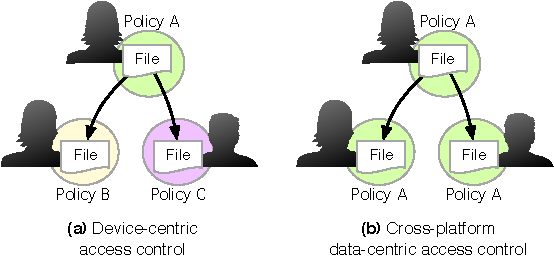
\includegraphics[width=\columnwidth]{fig/tcapsules-contrast.pdf}
    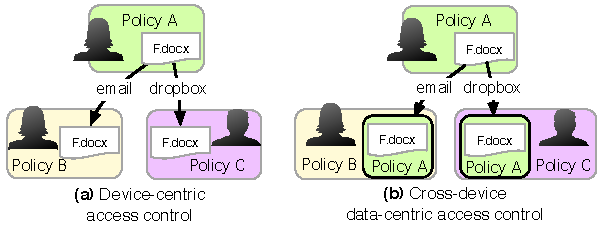
\includegraphics[width=\columnwidth]{fig/tcapsules-contrast2.pdf}
    \caption{(a) Today, a data creator has no control over their data on remote
      devices: devices enforce local policies on data they receive. We propose (b)
      cross-platform policies that move with data and are enforced uniformally
      across devices.}
    \label{fig:ControlBoundaries}
  \end{figure}
  %%%%%%%%%%%%%%%%%%%%%/
  
  Modern mobile devices are highly capable and have enabled users to create and
  share rich content such as videos, pictures, and documents. However, users often
  have little control over their shared data. As illustrated in
  Figure~\ref{fig:ControlBoundaries}, a user has full control over her file as
  long as it stays on her device. She loses this control the moment the file
  leaves her device boundaries. For example, files backed up to iCloud or Dropbox
  are vulnerable to the security of those platforms and files shared with other
  users are vulnerable to their benevolence and their device security policies.
  
  Users today rely on ad-hoc solutions. For example, they might use
  Cryptomator to encrypt their files before backing it up to the cloud
  or SnapChat to send self-destructing images that are viewable only for
  a limited period of time. These apps address particular use-cases with
  coarse controls and do not provide any general-purpose data protection
  mechanisms.
  
  Existing work has proposed several solutions to let users retain
  control over their data as it crosses device boundaries. A current
  state of the art approach is to use a hardware-based trusted
  execution environment (TEE) to control accesses to sensitive files.
  The focus is to ensure that users retain {\em full} control over their
  shared data. DroidVault~\cite{li14droidvault}, for example, does not
  allow regular apps running outside the TEE to access the
  data. Instead, it requires data owners to explicitly write and
  whitelist the code that is allowed to process sensitive data and it
  executes this code within the TEE. We believe that such restrictions
  make the corresponding systems impractical. Users already trust and
  rely on a variety of apps to create and share content. It is unlikely
  that users would use a system that does not support their apps.
  
  In this paper, we describe a platform-level file protection mechanism
  that does not restrict the apps users may use. To this end, we rely on
  a pragmatic pessimistic-optimistic threat model. In the pessimistic
  state, we consider the device and apps completely untrusted and rely
  on a TEE to perform safety checks. When it is considered safe, the
  system transitions into the optimistic state where we also trust the
  OS kernel and the app accessing sensitive data. Finally, when the app
  no longer uses the data, the system switches back into the
  pessimistic state. We leave a further discussion of our threat model
  to Section~\ref{sec:threat-model}.
  
  We contribute {\bf Trusted Capsules}, a data-centric access control abstraction that
  embodies the above threat model. It enables users to bundle sensitive files with
  flexible policies that govern their accesses into encrypted units we call {\em
    capsules}. Each capsule appears in the system as a regular file. When an app
  attempts to open a capsule, the platform evaluates the policy in a TEE. If the
  policy allows the access, the capsule's contents are unsealed (decrypted) and
  provided to the app and are resealed (re-encrypted) when the app later closes
  the file. In our prototype, we use ARM TrustZone as the TEE and design policies
  as stateful programs that can base access decisions on information such as
  location, time, or the number of prior accesses and may, if necessary, modify
  the data itself (e.g., for redaction).

  Our contributions may be summarized as follows:

\begin{itemize}

\item A pragmatic access control abstraction for protecting sensitive files
  across device boundaries that works with existing unmodified apps.

\item Using our prototype, we show that our proposed approach imposes slowdowns
  only when a capsule is being opened or closed (1.96x and 1.67x, respectively,
  using a no-op policy). Once a capsule file is open, data can be read at a
  throughput identical to reading regular files.

\end{itemize}


\endinput

Any text after an \endinput is ignored.
You could put scraps here or things in progress.


\chapter{Background}
\label{ch:Background}

{\bf ARM TrustZone}~\cite{trustzone} is a widely available hardware-based TEE
(Trusted Execution Environment) that partitions a device's CPU, memory, and
peripherals, into two isolated logical ``worlds'' --- normal and secure. Each
CPU core runs either in a non-secure state, where it has access only to
resources assigned to the normal world, or a secure state where it has access to
both normal and secure world resources. When switching between states (e.g., via
the {\tt smc} instruction), the secure monitor, a critical and heavily-vetted
software, is invoked to safely perform the transition. TrustZone enables a
trusted OS to run in the secure world in conjunction with an OS in the normal
world, and it protects state in the secure world even if the normal world is
compromised.

{\bf OP-TEE}~\cite{optee} is an open-source software stack that facilitates the
use of ARM TrustZone. It provides a secure world OS (OP-TEE OS) for executing
trusted applications; a low-level secure monitor for switching a core between
non-secure and secure states; a TrustZone driver for normal world OSes such as
Linux, which enables regular user-space applications to execute RPCs in the TEE;
and a user-space supplicant that enables applications running in the TEE to
access resources in the normal world OS.

\endinput
\chapter{Threat Model}
\label{ch:ThreatModel}
\begin{figure}
  \centering
%  \includegraphics[width=\columnwidth]{../Images/threat-model-state-diagram.pdf}
  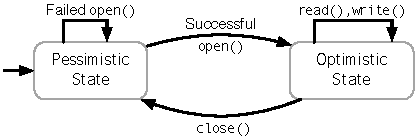
\includegraphics[width=\columnwidth]{fig/state-machine.pdf}
  \caption{A finite-state machine view of Trusted Capsule's threat model. Each
    capsule on a device begins in the pessimistic state. A successful transition
    from the pessimistic to optimistic state means an app on the device tried to
    open the capsule and the capsule's policy authorized the access. Only that
    app process is allowed to access that file in the optimistic state. When the
    process closes the file, the system transitions back to the pessimistic
    state.}
  \label{fig:threatmodelstatediag}
\end{figure}

Trusted Capsules use a contextual threat model. As illustrated in
Figure~\ref{fig:threatmodelstatediag}, this model has two states, {\em
  pessimistic} and {\em optimistic}, and there is a transition between
the two states depending on the context. We assume that device owners
have full control over the software stack running in the normal world
but may not modify the stack running within TrustZone.

The system begins in the {\em pessimistic} state, when the user first receives a
capsule on her device, which is encrypted data bundled with a policy that
governs its access. In this state, the TCB consists solely of ARM TrustZone and
the secure monitor; the OP-TEE OS running in TrustZone; and the Trusted Capsules
data monitor that runs in OP-TEE OS. All code running outside of TrustZone
(i.e., the normal world kernel and apps) are considered untrusted. In this
state, we guarantee that the capsule's decrypted contents are not available and
that it is safe from attempts to either exfiltrate or modify its data or
policies. When the user opens the capsule with an app (which will use the {\tt
  open()} syscall), the policy embedded in the capsule is executed by the
Trusted Capsules data monitor. If the policy denies access to the file, the
system remains in the pessimistic state (and the app's call to {\tt open()} will
fail).

If access is allowed, the system transitions to the {\em optimistic} state where
the decrypted capsule data is given to the app. The TCB in this state expands to
include the normal world kernel and the app that opened the file. Only that app
is authorized to access the file and we rely on the process isolation mechanisms
in the normal world kernel to prevent other unauthorized apps from accessing the
decrypted data. When the app closes the file (with the {\tt close()} syscall),
the capsule is re-sealed and the system transitions back to the pessimistic
state. If the app modifies the file before closing it, the changes are saved
only if allowed by the capsule policy. Otherwise, they are discarded.

We consider side-channel and analog attacks out-of-scope.

% We consider out-of-scope side-channel and analog attacks, and buggy or malicious
% capsule policies.

\subsection{Discussion}

% \iv{I would lead with table, and describe each scenario in context of
%   the relevant table cell.}
%
% \ar{Done.}

% \iv{I would move the table higher, and also not have it break up the
%   flow of your scenario.}
%
% \ar{Done.}

\begin{table}[ht]
  \small
  \begin{center}
    \begin{tabular}{|l|l|l|} \hline
      \diagbox{{\bf Adversary}}{{\bf State}}& Pessimistic & Optimistic \\
      \hline
      Weak & \Checkmark & \Checkmark \\
      \hline
      Strong & \Checkmark & \XSolid \\
      \hline
    \end{tabular}
  \end{center}
  \caption{An enumeration of the possible system state and adversary type
    combinations. The \Checkmark \ and \XSolid \ symbols indicate whether or not
    Trusted Capsules prevents data exfiltration in the corresponding
    scenario. Note that the adversary here is not authorized to directly open a
    capsule on the device.}
  \label{tab:trustedcapprot}
\end{table}

Table~\ref{tab:trustedcapprot} summarizes the protections Trusted Capsules
offers depending on the adversary's capabilities and the state of the
system. Consider the scenario when Alvin sends a capsule with a photo to
Barbara's smartphone with a policy that requires Barbara to authenticate herself
before she can view the photo. In the worst case, Barbara herself is an
adversary interested in leaking the photo. There are no mechanisms in Trusted
Capsules preventing Barbara from doing so; the best that can be done is for Alvin to
be sure he trusts Barbara before he authorizes her to view the photo.

Consider instead the situation where Barbara is trustworthy but her smartphone
is sometimes accessible by Charlie, an adversary who is secretly interested in
viewing Alvin's photo. Charlie's aim is to modify the state of the smartphone so
that when Barbara subsequently regains control of her phone and opens Alvin's
capsule, Charlie surreptitiously receives a copy of the photo.

If the system is in the pessimistic state, there is no way for Charlie to view
the photo because the capsule is sealed and encrypted. In the optimistic state,
whether Charlie can exfiltrate the photo depends on whether he is a {\em weak}
or a {\em strong} adversary. A weak adversary is one who is not technically
inclined and hence may not do much more than install new apps from the
smartphone app store. In this event, when Barbara opens the capsule and the
system switches to the optimistic state, Trusted Capsules relies on the kernel's
app isolation mechanisms to prevent other unauthorized apps Charlie might have
installed from accessing the decrypted capsule data.

On the other hand, if Charlie is a strong adversary, then he may use a variety of
techniques such as kernel modifications to access the photo in the optimistic
state. While Trusted Capsules does not protect against this scenario at the
moment, it may be mitigated by having the policy reason about the normal world
software stack before opening the capsule. We leave an investigation of this
strategy to future work. Finally, note that regardless of the system state and
adversary type, an adversary may not alter the policy embedded in a capsule and
it never leaves the TrustZone environment.

% \iv{I think the state machine view that we drafted on the whiteboard
%  is missing to connect the 'transition' between these. i.e., the
%  'states' are actual states in a state machine. I think we need to
%  add the FSM to make this more clear. It will also help the
%  description above.}
%
% \ar{Added the state diagram above. Hopefully this makes the explanation
%  clearer.{

\chapter{Trusted Capsules}
\label{ch:trustedcapsules}
At a high-level, Trusted Capsules packages data into protected units known as
    {\em capsules}. When an app in the normal world tries to open a capsule, the
Trusted Capsules data monitor intercepts the open and executes the policy within
the TrustZone TEE. If the capsule's policy authorizes the access, the capsule
data is decrypted and returned to the app. When the application eventually closes the file,
the data monitor re-seals the capsule, evaluating another on-close policy
to determine e.g., whether capsule content can be mutated. In the rest of this section,
we describe the components of our system.

\section{Capsules}

%%%%%%%%%%%%%%%%%%%%
%% \ref{fig:trustedcapsulelayout}
\begin{figure}
    \centering
    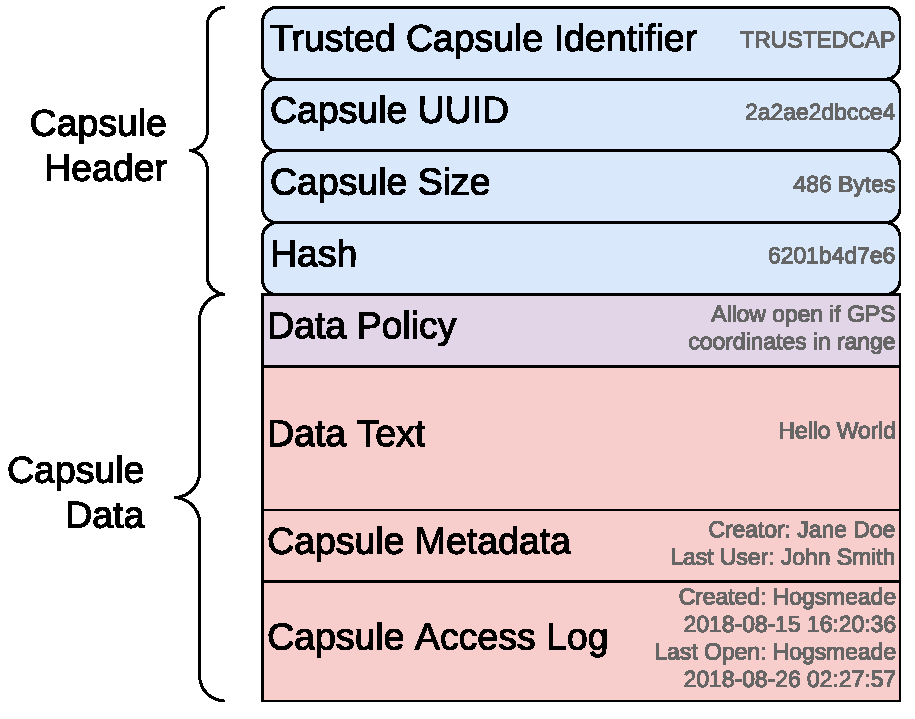
\includegraphics[width=\columnwidth]{fig/Fig2_Trusted_Capusle_Layout_New.pdf}
    \caption{Trusted capsule layout.}
    \label{fig:trustedcapsulelayout}
\end{figure}
%%%%%%%%%%%%%%%%%%%%

A capsule consists of data and an access policy for the data, both encapsulated
into a single encrypted file. Figure~\ref{fig:trustedcapsulelayout} illustrates
the format of a capsule. A capsule has an unencrypted header segment followed by an
encrypted data block. The header identifies the file as a capsule and contains
integrity metadata used by the data monitor, such as a hash of the contents of
the data block before they were encrypted. The data block contains the protected
data, its access policy, and metadata associated with the policy, such as access
logs. We assume that the cryptographic keys required to decrypt capsules are
securely loaded into a secure storage area accessible only by the TEE.
%
%\iv{Have to differentiate between on-open and on-close policies.}

\section{Policy API}
\label{subsec:policy}

% Please add the following required packages to your document preamble:
% \usepackage{booktabs}
% \usepackage{graphicx}
\begin{table}[]
    \centering
    \resizebox{\textwidth}{!}{%
    \begin{tabular}{@{}|l|l|@{}}
    \toprule
     & \textbf{Description} \\ \midrule
    \multicolumn{2}{|l|}{\textbf{Open-Only}} \\ \midrule
    {\tt redact}({\em start}, {\em end}, {\em replaceBytes}) & Replace byte range [{\em start}, {\em end}] of trusted capsule data with bytes {\em replaceBytes}. \\ \midrule
    \multicolumn{2}{|l|}{\textbf{Close-Only}} \\ \midrule
    {\tt readNewCapsuleData}({\em offset}, {\em length}) & Return {\em length} bytes from {\em offset} of new trusted capsule data. \\ \midrule
    {\tt newCapsuleLength}() & Return the length of new trusted capsule data. \\ \midrule
    \multicolumn{2}{|l|}{\textbf{Shared}} \\ \midrule
    {\tt getState}({\em key}, {\em where}) & Get state mapped to {\em key} from {\em where}. \\ \midrule
    {\tt setState}({\em key}, {\em val}, {\em where}) & Set state mapped to {\em key} to {\em val} in {\em where}. \\ \midrule
    {\tt getLocation}({\em where}) & Get location of device from {\em where}. \\ \midrule
    {\tt getTime}({\em where}) & Get current time from {\em where}. \\ \midrule
    {\tt readOriginalCapsuleData}({\em offset}, {\em length}) & Return {\em length} bytes from {\em offset} of original trusted capsule data. \\ \midrule
    {\tt originalCapsuleLength}() & Return the length of original trusted capsule data. \\ \midrule
    {\tt deleteCapsule}() & Delete the trusted capsule. \\ \midrule
    {\tt updatePolicy}() & Check for policy update with trusted capsule server. \\ \midrule
    {\tt appendToBlacklist}({\em key}, {\em where}) & Append {\em key} to blacklist of {\em where} - used by log to prune states in {\em where}. \\ \midrule
    {\tt removeFromBlacklist}({\em key}, {\em where}) & Remove {\em key} from blacklist of {\em where}. \\ \bottomrule
    \end{tabular}%
    }
    \caption{The Lua-based API that policies in Trusted Capsules may use}
    \label{Tbl:lua_ext}
    \end{table}
    
In Trusted Capsules, policies are written in the Lua programming language and
have one simple requirement: they must implement an {\tt evaluate\_policy}({\em
        op}) function that is called when the capsule is being opened or closed; the
    {\em op} argument distinguishes between the two. In either case, the function
has to return a boolean value that is interpreted differently depending on the
operation. If it returns {\tt true} on a capsule open, the data is decrypted and
given to the normal world app. Otherwise, access is denied. On a capsule close,
returning {\tt true} means file modifications by the normal world app will be
kept while {\tt false} means they will be discarded. Policies may also use the
Trusted Capsules API listed in Table~\ref{Tbl:lua_ext} to easily perform common
operations:

\textbf{Storing state}: Policies may store and retrieve arbitrary state using
the state-oriented APIs such as {\tt getState} and {\tt setState}. When using
such methods, the policy must specify {\em where}
state is to be kept. A policy may securely store state in the metadata space within
its capsule, in external secure storage, or at a remote server. If a policy
communicates with a remote server, the networking stack in the normal world
kernel is used to initiate the connection. However, as the OP-TEE OS includes
the mbed TLS library~\cite{mbed}, it is possible to safely make an HTTPS
connection from the secure world without trusting normal world.

\textbf{Ensuring data integrity}: Our Lua policy provides APIs to retrieve the
original trusted capsule data at file open (read) and the new trusted capsule
data at file close (write). Using these APIs, data owners can express
policies that, for example, protect specific data regions from being
overwritten. %%  \ar{This explanation is incomplete. How exactly does one prevent
%% specific regions from being overwritten?}

\textbf{Redaction}: Selective policy-based disclosure of trusted capsule
contents is a key feature of trusted capsules. Using our byte-oriented
redaction API, data owners can express arbitrary data
transformations on regions of the data based on the environment and
the state of the device \emph{prior to} disclosing information to the normal world.  Examples
of data transformations include removing sensitive texts or blurring
images. %  \ar{Probably should merge this and data integrity section together.}

\textbf{Revocation}: A policy can specify revocation in two
ways. First, we provide APIs to allow policies to self-delete a trusted
capsule. When the \textit{deleteCapsule} API is called, we overwrite
the trusted capsule file with zeros\footnote{This is because the Linux OS does not
    actually delete the file until the file's reference count becomes zero}. We then
make an RPC call into the normal world to delete the file and destroy the
trusted capsule application session. Such a revocation is permanent.  Second, we
allow retroactive policy changes via the remote capsule server. In this
scenario, the policy specifies a condition under which \textit{updatePolicy} is
called. If a new policy exists at the trusted capsule server, it is downloaded
by the trusted world and replaces the prior policy. Policy changes are temporary as the owner
could always change the policy back. %% With trusted capsules, revocation can be gradual
%% based on user needs.
%% \ar{This portion is
%%   weak. The {\tt deleteCapsule} method is easily defeated. If someone sends me
%%   an email with a capsule, and I find the capsule revoking itself, couldn't I
%%   just download a copy of the capsule again? What's the utility of
%%   deleteCapsule?}

\textbf{Logging}: We extended the Lua language with the ability to report
information to the remote capsule server. To enable logging on open and close, \textit{log\_open}
and \textit{log\_close} flags must be set to true, respectively.
By default, the Lua sandbox will report the location,
identity, time, and the operation. Additional local or capsule state information are
also logged, unless otherwise specified by the APIs \textit{appendToBlacklist}
and \textit{removeFromBlacklist}. The logs are written into the LOG section of
the trusted capsule.  If the section runs out of space, the logs are flushed to
the remote server and then overwritten. %% \ar{Is this really necessary as a
%% separate paragraph? The access log isn't used for anything special, so why not
%% have it part of the {\tt getState} and {\tt setState} API? Alternatively, add
%% the logging API methods to the table and just highlight the usefulness of that
%% here.}


\section{Data monitor}

%%%%%%%%%%%%%%%%%%%%
\begin{figure}
    \centering
    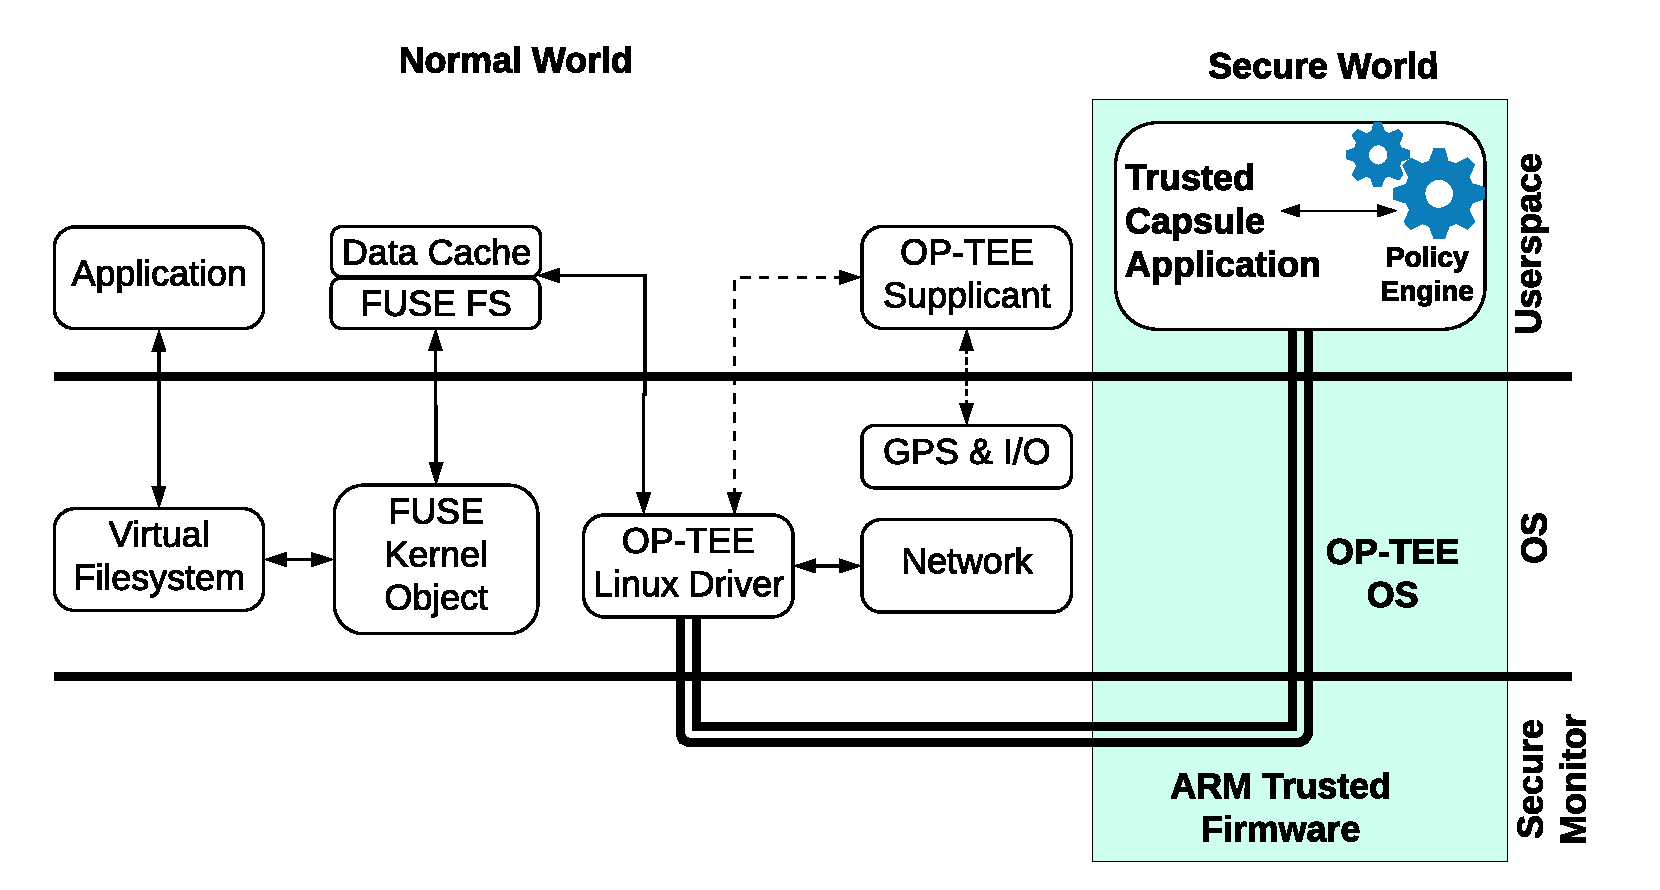
\includegraphics[width=\columnwidth]{fig/Fig3_TC_data_monitor_system_cache.pdf}
    \caption{Trusted capsule data monitor design. Application system calls to the filesystem for accessing trusted capsules are intercepted and forwarded to the trusted capsule application through the FUSE filesystem and OP-TEE Linux Driver.
        The secure world trusted capsule applications access peripheral I/O through RPC calls to the OP-TEE Supplicant via the OP-TEE Linux Driver.}
    \label{fig:SystemModel}
\end{figure}
%%%%%%%%%%%%%%%%%%%%

%%%%%%%%%%%%%%%%%%%%
\begin{figure*}
    \centering
    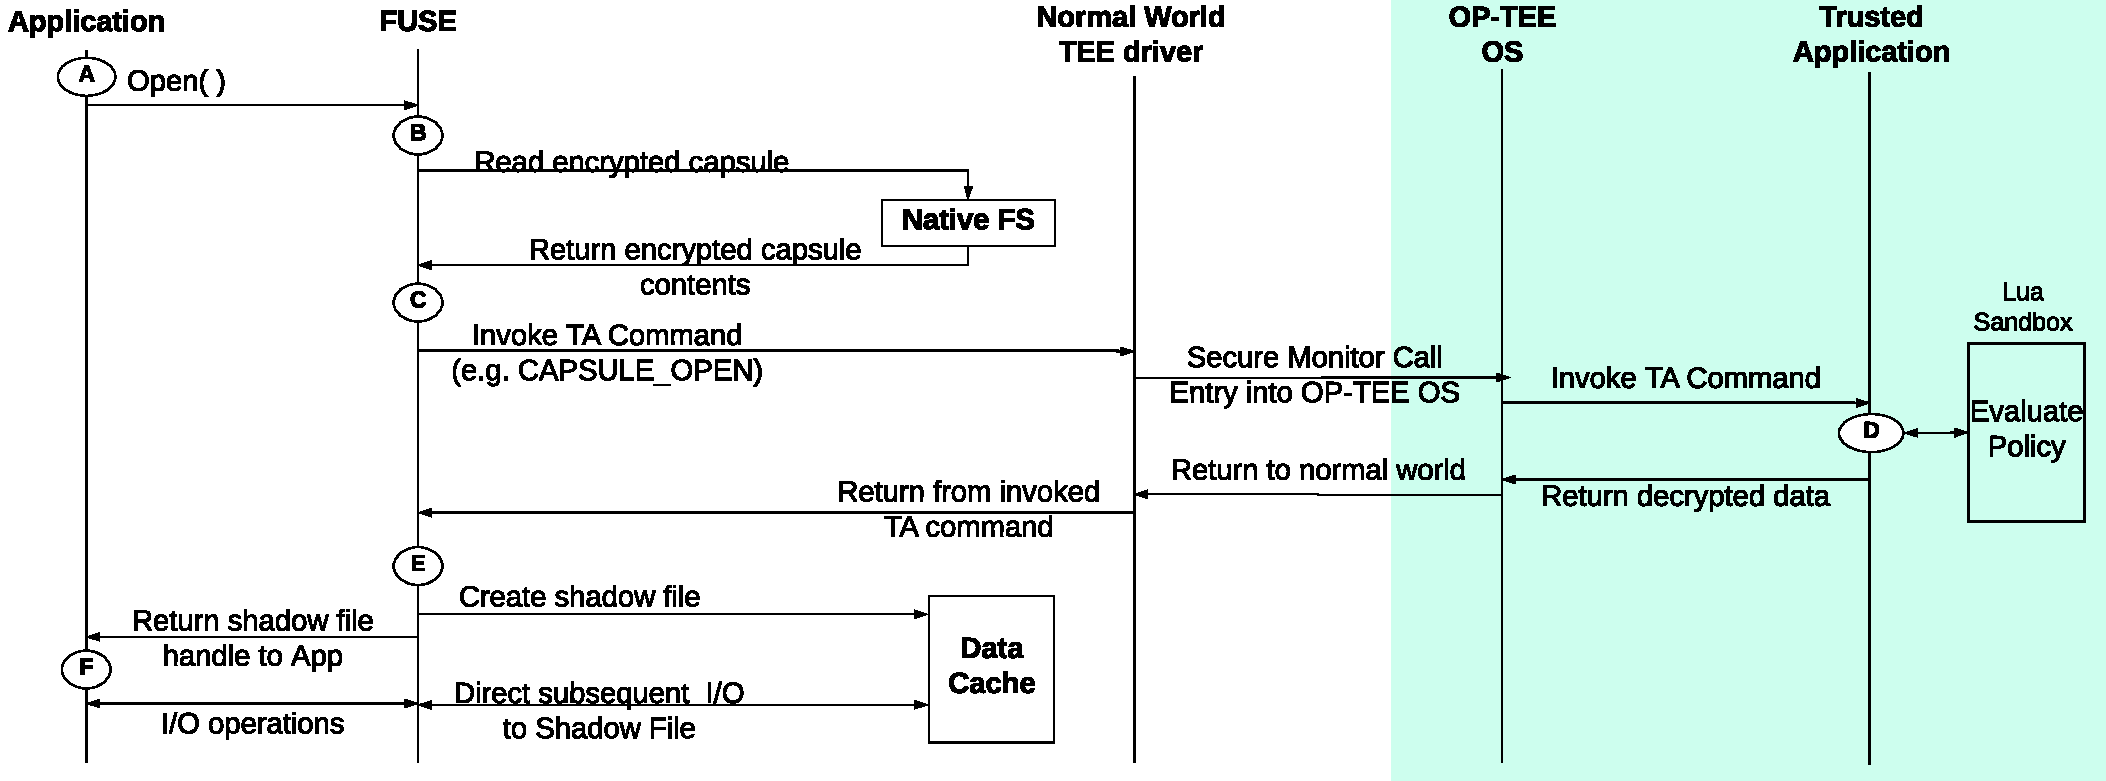
\includegraphics[width=\textwidth]{fig/TC_open_operation.pdf}
    \caption{Trusted capsule monitor operation (shaded region operates in the secure world).
        \textbf{A.} Application \textit{open} system call is intercepted.
        \textbf{B, C.} FUSE identifies if a file is a capsule, and if so, invokes an RPC into the secure world to decrypt the capsule.
        \textbf{D.} The trusted capsule application (TA) evaluates the \textit{open} policy.
        \textbf{E.} FUSE writes the decrypted contents to a shadow file
        \textbf{F.} The application is returned a filehandle to the shadow file, and all subsequent I/O requests are directed to the shadow file.
    }
    \label{fig:FlowChart}
\end{figure*}
%%%%%%%%%%%%%%%%%%%%

In Figure~\ref{fig:SystemModel}, we illustrate the different components of the
data monitor in our system and in Figure~\ref{fig:FlowChart}, we show a detailed
data flow between them when an application opens a capsule. These components may
be broadly classified into (1) framework code that runs in the normal world OS,
and (2) a policy execution engine in the secure world. Next, we discuss
each component in detail while referring to the data flow in
Figure~\ref{fig:FlowChart}.

{\bf Normal world framework}: We implemented a passthrough FUSE filesystem in
the normal world and expose it as a separate mount point. When an application
opens files located on this mount point, our framework will interpose on the
application's {\tt open} syscall. It will check the header of the file to
identify if it is a capsule. If it is a regular file, it will just load the raw
file from the underlying file system and return it to the app.

If it is a capsule, the file contents are copied into a memory buffer. FUSE then
shares this buffer with the policy execution engine running inside secure world
and invokes the engine's {\em decrypt} function ({\em A}-{\em C} in
Figure~\ref{fig:FlowChart}). If the policy authorizes the access, the policy
engine will return the decrypted contents of the capsule and FUSE will save them
into a shadow file ({\em E}). It will subsequently return a handle to this
shadow file to the application ({\em F}). Hence, all reads and writes to the
capsule by the application will be transparently redirected to the shadow file.

When the application closes the capsule, FUSE copies the shadow file back into a
shared buffer, sends it to the policy execution engine, and invokes the {\em encrypt}
operation. This returns the reconstructed capsule, with the updated policy
metadata and data contents (as authorized by the policy), which is then written
in place of the original capsule file.

Our framework prevents multiple applications from concurrently opening the same
capsule. This simplifies the design of our data monitor as we do not have to
reason about multiple-reader/multiple-writer type problems when saving a
capsule. An application may, however, have multiple capsules open.

    {\bf Policy execution engine}: We implemented a Trusted Application (TA) that
runs within OP-TEE OS in secure world. It contains a Lua interpreter, to execute
a capsule's policies, and it is responsible for maintaining the runtime session
state associated with a capsule (e.g., cryptographic keys) and updating the
capsule metadata.

When a {\em decrypt} operation is received from the normal world (because a
normal world application used the {\tt open} syscall on a capsule), a new
instance of the trusted application is started. It (1) loads the capsule, (2)
loads the cryptographic keys for the capsule, (3) executes the policy, and (4)
returns the decrypted capsule data if authorized by the policy. During policy
evaluation, it may communicate to a remote server directly from secure world.

On an {\em encrypt} operation (which is initiated because a normal world
application used the {\tt close} syscall to close a capsule), the TA evaluates
the policy and provides it the opportunity to allow or deny modifications to the
capsule data. Next, it updates the metadata, produces a new capsule file with
updated contents in the data block, and updates the integrity metadata in the
header. Finally, the reconstructed capsule is given to the normal world for
storage and subsequent use.

%%%%%%%%%%%%%%%%%%%%
% \begin{figure}
%   \centering
%   \includegraphics[width=\columnwidth]{../Images/TrustedApplicationSession.pdf}  
%   \caption{Trusted capsule monitor session model. Each Trusted Capsule Application maintains the session for
%            a single trusted capsule. It supports multiple file handles per trusted capsule. The file handles
%            consists of the process ID and file descriptor.}
%   \label{fig:trustedapplicationsession}
% \end{figure}
%%%%%%%%%%%%%%%%%%%%	

% Each instance of the trusted application independently maintains a trusted
% capsule's session state. \textbf{Session states include the \emph{cryptographic
%     and hashing handles, role-based credentials, hashes of the trusted capsule
%     contents, and copies of the data and policy}}. Further, the trusted
% application acts as the \textbf{endpoint for secure communication with a trusted
%   capsule server for performing remote functions} (e.g., fetching remote state
% or initiating a policy change). The trusted capsule application handles
% sensitive information and performs critical functions that must be protected
% against the untrusted normal world. Therefore we require this part of the
% trusted data monitor to execute within TrustZone.

We use OP-TEE OS native secure storage capability to store our cryptographic
keys and persistent trusted capsule states. Cryptographic information is stored
in serialized binary while trusted capsule states are stored in key-value
format. All trusted capsule encryption keys are stored in a single secure key
file. We allow the key file to be accessible by multiple trusted capsule
applications at a time so that multiple sessions can be instantiated
simultaneously to handle different capsules. In contrast, each capsule get its
own secure state file. State files can only be opened by a single trusted
capsule application at a time. This is enforced through the OP-TEE OS. In this
way, we enforce a single trusted capsule instance at a time per capsule.

% Trusted application methods are invoked by FUSE based on specific system
% calls. In this way, access control can be enforced dynamically based on the
% local and remote state when such a system call is initiated. We describe several
% of these methods below.

\section{Security analysis}

We consider two important security aspects of the Trusted Capsules data monitor.

\textbf{Trusted Capsules}: Operations on the trusted capsule are performed by
the trusted application in the secure world. We isolate each trusted capsule by
having separate instances of the trusted application handle each capsule and
by relying on OP-TEE OS to isolate each trusted application instance.
Our system stores persistent state associated with capsules (such as cryptographic keys)
in secure storage using OP-TEE.

Given our use of TrustZone, the confidentiality and integrity of the capsule
data is protected against compromises of the normal world OS, particularly in
the pessimistic state. A compromised normal world OS may corrupt a capsule, but
that corruption will be detected during decryption. In the worst case, a compromised OS
may leak the data of capsules that are open during the compromise.

\textbf{Policy Evaluation}: To account for malicious policies, we made several
changes to the Lua interpreter to make it a sandbox. We disabled any Lua library
that allows the interpreter to interact with external systems (e.g., I/O,
packages, debug, and OS). We also extended the interpreter to prevent policies
from (1) interacting with any files other than the capsule, (2) from accessing
keys associated with other capsules, and (3) reading unauthorized device
peripherals. A malicious policy may attempt denial-of-service attacks such as
infinite loops. However, these may be addressed even by the normal world, by
canceling an {\em encrypt} or {\em decrypt} commands that do not complete after
some time.

%%%%%%%%%%%%%%%%%%%%%%%%%%%%%%%%%%%%%%%%%%%%%%%%%%%%%%%
\chapter{Use case examples}
\label{sec:new-policies}
%%%%%%%%%%%%%%%%%%%%%%%%%%%%%%%%%%%%%%%%%%%%%%%%%%%%%%%

In this section, we discuss several use cases to highlight the capabilities of
Trusted Capsules.

% In this section, we introduce four policies that demonstrate how trusted
% capsules can be used in real-life scenarios that require the enforcement of
% strong first-use policies. We use these policies to evaluate the system in
% section \ref{sec:eval}, and to demonstrate the expressiveness of our policy API
% as introduced in Section \ref{subsec:policy}.


\textbf{Access control based on time or location}: Enterprises may wish to
restrict employees from opening company files outside the office or a user may
require his family members to only view shared pictures at their
homes. Alternatively, the data owner may wish to allow access to sensitive
content only within a pre-determined time period. Such requirements are
straightforward to express in our system. When a capsule policy's
\texttt{evaluate\_policy()} function is evaluated at the time of
\texttt{open()}, it can access the device location and time to decide if the
access should be allowed or denied. Alternatively, instead of simply denying access
to a capsule, policies may use the \texttt{redact()} API in
Table~\ref{Tbl:lua_ext} to allow access but with sensitive content
redacted.

For example, Figure~\ref{fig:location_policy} illustrates a policy
that denies access to the capsule if the location from which it is
being accessed is outside the specified location range. 

\textbf{Requiring permissions in real time}: In some cases, users may wish to
have real time control over their data. For example, Alvin may wish to be asked
each time Barbara opens his capsule whether or not to allow her access. It is
straightforward to support this scenario in Trusted Capsules as policies can
communicate with remote servers over the Internet.

We implemented this scenario in our prototype using Twitter. When a user opens a capsule,
the policy uses the \texttt{getState()} API method to communicate with a custom
server and passes the Twitter handle of the capsule owner. The server then sends
a direct Twitter message to the owner of the capsule with an access request
and asks him to respond with a ``yes'' or ``no'' to approve or decline the access,
respectively. The server returns the owner's decision to the policy and the
appropriate action is taken. At the moment, the Twitter message to the owner
does not identify the user trying to open the capsule but this can be
implemented by mapping unique device identifiers to Twitter handles.

\textbf{Progressive trust}: The APIs in Table~\ref{Tbl:lua_ext} may be composed
to support other useful scenarios. Suppose Bob wants to share
sensitive data with someone but does not yet completely trust that person. He
can use a policy that contacts a remote server to log access attempts and to
identify what data should be returned to the app. Initially, Bob may choose to
provide a heavily redacted version of the data (e.g., an image with blurred-out
faces or a document with key sections removed). As his trust towards
the person grows, he can progressively share more sensitive content by recording his
decisions on the server.

% \textbf{Pre-distribution of content}: Popular TV shows such as Game of Thrones
% suffer from massive bandwidth load during their premier nights on video
% streaming services. Ideally, creators should be able to write policies that
% allow them to pre-distribute their content while ensuring that it cannot be
% viewed until a pre-set release date.

As an example of a policy with progressive trust, consider
Figure~\ref{fig:time_based_access} which consider content
pre-distribution: a capsule creator writes this policy to
pre-distribute their content while ensuring that the content cannot be
viewed until a pre-set release date. For this use case, we rely on a
trusted remote server for getting the time. Capsule metadata is first
inspected using \texttt{getState()} to check if the content has
already been approved for access by the policy. If this is indeed the
first access to the capsule, using the \texttt{getTime()} API, the
remote server is contacted to get the epoch value and it is compared
to the epoch value in the policy. If the remote epoch stamp is greater
than the time encoded in the policy, the access is approved, and the
metadata is updated using \texttt{setState()} to reflect this. Any
subsequent accesses to the capsule do not involve querying the remote
server for getting the time.

% In situations where the data-owner wishes to exercise greater control over who
% gets to access their data, relying on such statically defined policies might not
% be an appealing solution. Data owners might want to push new policies to affect
% change in capsules that have already been created and circulated.  This use-case
% can be serviced by using the trusted server to host new policy versions. The The
% \texttt{updatePolicy()} API can be used by the trusted application to get an
% updated version from the remote server.

% This mechanism, however, has an inherent delay between the when the owner
% decides to change the policy for a capsule, and the change getting published
% since it is contingent on the owner writing and releasing a new policy
% version. This non-trivial amount of work can lead to the data owners not
% updating the policies in time.

% A mechanism for asking the owner for access in real-time could alleviate this
% effort and provide a finer-grained control on data access. To this end, we
% extended the policy API to introduce a new remote location to seek permission
% from - Twitter. The data owner embeds her Twitter handle in the policy and sets
% the location for metadata operation to "POLICY\_REMOTE\_SERVER". The key for the
% \texttt{getState()} operation is set to "twitter:<username>". The "twitter:"
% string in the key is used to distinguish this as a Twitter request.

% When the remote server receives a \texttt{getState()}, and identifies the key to
% be a twitter handle, it invokes the Twitter Direct Message API to send an open
% request to the data owner. When the data owner receives this response, they can
% reply to "yes" or "no" to approve or decline the access request
% respectively. The server then returns the response to the Trusted Application
% which then returns the appropriate action.

% \textbf{Allowing access to data in agreed upon locations}: This policy can be
% used by data-owners to control \emph{where} their data can be
% accessed. Enterprises may wish to exercise control on where their employees may
% be able to access their sensitive data.
% {
% \pu{We need to identify why simply
%   blocking access to copying data does not work - This is usually done by using
%   device-level policies that block ways which can be used to copy the data, say,
%   blocking access to USB media.}

\begin{figure*}[t]
\begin{lstlisting}[language={[5.1]Lua} ,basicstyle=\small,showstringspaces=false,numbers=left,stepnumber=1,tabsize=1]
longitude = 1250
latitude = 200
range = 10

function evaluate_policy( op )
    if op == POLICY_OP_OPEN or op == POLICY_OP_CLOSE then
        long, lat, err = getLocation( POLICY_LOCAL_DEVICE )
            if err ~= POLICY_NIL then
                comment = "Failed to getLocation"
                return false
            end
            if math.abs(long - longitude) <= range
            and math.abs(lat - latitude) <= range then
                comment = "GPS coordinates in range"
                return true
            else
                comment = "GPS coordinates are not in range"
                return false
            end
    end
end
\end{lstlisting}
\caption{Simple location based access policy}
\label{fig:location_policy}
\end{figure*}


% \textbf{Location based redaction}: The policy as specified is fairly restrictive
% and blocks all access to the data contents outside a geographical range. There
% can be a scenario where the data owners wish to allow the partial revelation of
% the data in locations that are not trusted. To fulfill this requirement, the
% policy in Figure \ref{fig:location_policy} can be tweaked to allow redaction of
% data that is marked confidential by the creator.

% The data creator can encapsulate sensitive information in the data within some
% policy defined secrecy tags (for example: \texttt{<secret> , </secret>} can be
% used). The \texttt{redact()} API can be used in the policy to look for these
% tags and replace the text contained therein with a replacement string. This
% policy is shown in Figure \ref{fig:location_redaction_policy}.

% \begin{figure}
% \begin{lstlisting}[language={[5.1]Lua} ,basicstyle=\tiny,showstringspaces=false,numbers=left,stepnumber=1,tabsize=1]
% replaceVar = "REDACTED"
% longitude = 1250
% latitude = 200
% range = 10
% startTag = "<secret>"
% endTag = "</secret>"
% function evaluate_policy( op )
%     if op == POLICY_OP_OPEN or op == POLICY_OP_CLOSE then
%         long, lat, err = getLocation( POLICY_LOCAL_DEVICE )
%         if err ~= POLICY_NIL then
%             policy_result = POLICY_NOT_ALLOW
%             comment = "Failed to getLocation"
%             return
%         end
%         if math.abs(long - longitude) <= range
%         and math.abs(lat - latitude) <= range then
%             comment = "GPS coordinates in range"
%             policy_result = POLICY_ALLOW
%             return
%         else
%             comment = "GPS coordinates are not in range. Redacting data."
%             policy_result = POLICY_NOT_ALLOW
%         end
%         while s ~= nil and e ~= nil do
%             s = string.find(data, startTag, s)
%             if s ~= nil then
%                 e = string.find(data, endTag, s+1)
%                 if e ~= nil then
%                     err = redact( s, e, "replaceVar" )
%                     if err ~= POLICY_NIL then
%                         policy_result = err
%                         return
%                     end
%                 end
%             end
%         end
% \end{lstlisting}
% \caption{Location based redaction policy}
% \label{fig:location_redaction_policy}
% \end{figure}

% \textbf{Pre-distribution of content}: Popular TV shows such as Game of Thrones
% suffer from massive bandwidth load during their premier nights on video
% streaming services. Ideally, creators should be able to write policies that
% allow them to pre-distribute their content while ensuring that it cannot be
% viewed until a pre-set release date.

% This use-case can be expressed easily in our policy API. To facilitate this use
% case, we rely upon a trusted remote server for getting time. Capsule metadata is
% first inspected using \texttt{getState()} to check if the content has already
% been approved for access by the policy. If this is indeed the first access to
% the capsule, using the \texttt{getTime()} API, the remote is contacted to get
% the epoch value and it is compared to the epoch value in the policy. If the
% remote epoch stamp is greater than the time encoded in the policy, the access is
% approved, and the metadata is updated using \texttt{setState()} to reflect
% this. Any subsequent accesses to the capsule do not involve querying the remote
% server for getting the time.

\begin{figure*}[t]
\begin{lstlisting}[language={[5.1]Lua} ,basicstyle=\small,showstringspaces=false,numbers=left,stepnumber=1,tabsize=1]
-- remote server information
remote_server = "198.162.52.127:3490"
-- return keywords
policy_result = POLICY_NOT_ALLOW
comment = ""

-- policy-specific keywords
open_time = 1523338041
opened = "opened"

function evaluate_policy( op )
    if op == POLICY_OP_OPEN then
        r, err = getState( opened, POLICY_CAPSULE_META )
        if r == "true" then
            return true
        else
            curr_time, err = getTime( POLICY_REMOTE_SERVER )
        end
        if err ~= POLICY_NIL then
            policy_result = err
            comment = "Failed to get time from remote server"
            return false
        end
        if curr_time > open_time then
            err = setState( opened, "true", POLICY_CAPSULE_META )
            if err ~= POLICY_NIL then
                policy_result = err
                comment = "Failed to update capsule metadata"
                return false
            end
            return true
        end
    end
end
\end{lstlisting}
\caption{Policy to allow content pre-distribution}
\label{fig:time_based_access}
\end{figure*}

% This policy can also be easily tweaked to revoke access to the file after a pre-determined amount of time has elapsed since the first time the capsule was successfully accessed. In this scenario, the default policy action is \texttt{POLICY\_ALLOW} and the policy transitions to the \texttt{POLICY\_NOT\_ALLOW} once the view window expires. Such a policy can be useful when sharing documents, for instance - college transcripts, that contain sensitive personal identifiers like Social Security Numbers (SSNs).
 %--paper 
%%%%%%%%%%%%%%%%%%%%%%%%%%%%%%%%%%%%%%%%%%%%%%%%%%%%%%%%%%%%%%%%%%%%%%%%%%%%%%%%
\chapter{Prototype}
\label{sec:implement}
%%%%%%%%%%%%%%%%%%%%%%%%%%%%%%%%%%%%%%%%%%%%%%%%%%%%%%%%%%%%%%%%%%%%%%%%%%%%%%%%

We prototyped Trusted Capsules on a LeMaker HiKey development
board~\cite{hikey}. It has an octa core ARM Cortex-A53 processor, 2~GB
of RAM, 8~GB of flash storage. and it comes with TrustZone unlocked,
thereby allowing us to control what OS runs on the TEE. We use Linaro
OP-TEE OS (version 3.3) in TrustZone and a HiKey Debian OS (based on
Linux 4.4.15) in the normal world. We modified the OP-TEE OS to
implement several missing {\tt libc} functions (such as {\tt atoi} and
{\tt strcmp}). As the HiKey board does not have a GPS receiver, we
mocked a GPS device that returns predefined longitude and latitude
values.

Capsules are encrypted with 128-bit AES. We consider the distribution
of keys required to decrypt capsules outside the scope of this paper.

Our data monitor is written in C and consists of about 6.2K SLOC: the
policy execution engine, which runs within the TEE, has about 4.2K
SLOC while the normal world framework has 2K.

%%%%%%%%%%%%%%%%%%%%%%%%%%%%%%%%%%%%%%%%%%%%%%%%%%%%%%%%%%%%%%%%%%%%%%%%%%%%%%%%%%%%%
\subsection{Prototype Evolution}\label{sub:proto-prototype}
%%%%%%%%%%%%%%%%%%%%%%%%%%%%%%%%%%%%%%%%%%%%%%%%%%%%%%%%%%%%%%%%%%%%%%%%%%%%%%%%%%%%%

The system design and the prototype evaluated in this paper has
evolved from a previous design of the system. This prior system
(``version-0'') had the ambitious goal of evaluating a Lua-based
policy in TEE on all intercepted file I/O system calls on a capsule
file: \texttt{open}, \texttt{close}, \texttt{read}, \texttt{write},
and \texttt{lseek}. As well, Version-0 revealed \emph{chunks} of the
file to normal world applications, rather than decrypting and
revealing the entire file contents on \texttt{open}. Version-0 was not
based on FUSE, but it used a custom system call interceptor in the
normal world OS. This interceptor worked in a manner similar to the
FUSE filesystem in our current design

Version-0 prototype was mature and stable, but had to be abandoned
because of unacceptable application slowdown. This was due to the
invasive nature of the system call handler that slowed down the
behaviour of most applications that open and close many files at
start-up. 

More concretely, the time to open a small document under a no-op
policy with FUSE on our hardware is 24ms, %\iv{.5s}
while the latency in Version-0 was 1.2s. %\iv{5s}. 
This is a speed-up of 50x over Version-0.

%By contrast, in our current prototype the
%latency is \iv{1s}, which is a speed up of \iv{5x} over Version-0. 

The latency and throughput gap dramatically increased for large and
complex file types, such as PDF JPEG. This can be observed in the raw
video footage for several use-cases in Version-0 of the system:
\url{https://goo.gl/SiBEJB}.

We note that while overhead in Version-0 was significantly better at
the application layer as compared to the system call layer,
nevertheless, the cost was prohibitive and was tightly connected to
the policy being used.
%
%% %% For various data types, a null
%% %% policy had much less significant or almost imperceivable impact to
%% %% usability at the application level. However, 
%% our use-case policies, some of which contained expensive policy checks
%% (e.g., access to state storage or going over the network to talk to
%% the policy coordinator) on frequent operations such as read or write,
%% resulted in noticeable performance degradation.
%
For example, our MP4 video played smoothly with a null policy in VLC
(which did not interact with the trusted capsule server), but degraded
to extreme jitter once we added a policy that reported actions to a
policy coordinator and accessed secure storage for every read
operation. This effect was particularly acute for the PDF reader,
which repeatedly read the data in small chunks frequently and even
when the user was idle. Each read by the PDF incurred the cost of a
single round-trip to the trusted capsule server, requiring on average
5ms each. 

Our experiences with Version-0 of the Trusted Capsules prototype have
been our guiding principle in making our current system perform
better.
%
Our benchmarking results (presented in the next Section) indicate that
the current Trusted Capsules design, that evaluates policy exclusively
on \texttt{open} and \texttt{close} calls strikes a better trade-off
between security and performance.


%% Our prototype
%% supports the following composable policy actions:

%% \begin{itemize}

%% %\item Allowing or denying the operation on the trusted capsule.

%% \item Allowing or denying the capsule to be opened or modified based on various
%%   signals such as location, time, or device identity.

%% % \item Reporting the operation, location, time, role-identity of the
%% %   device to a global policy coordinator.

%% \item Logging capsule accesses and reporting them to a remote server.

%% %\item Initializing or modifying persistent state (e.g., counter).

%% \item Initializing or modifying persistent capsule metadata (e.g., counter).

%% % \item Performing byte-based or keyword-based redaction that partially
%% %   discloses trusted capsule data. %A data-type specific pre-processor
%% %   %can be used to generate the byte offsets.

%% \item Performing byte-based or keyword-based redaction that partially discloses
%%   trusted capsule data. \ar{Table~\ref{Tbl:lua_ext} doesn't list the API to
%%     perform keyword-based redaction.} \pu{all redaction is based on byte offsets. the keyword search happens in lua and then the byte offsets are passed to the C API. How should I phrase this then?}

%% \item Hard access revocation by deleting the capsule, triggered
%%   locally or remotely; and, gradual access revocation based on evolving policy decisions that are adaptive to context of access - for example, total number of accesses, passage of time, policy updation, etc.
%%   %soft revocation by arbitrarily changing
%%   %the policy. 
%%   \ar{What's soft revocation?}\pu{Check}

%% % \item Prevent declassification through the network or file system.


%% %\item Registering a callback -- to place a deterministic real-time bound on when a policy is re-evaluated
%% %\item Killing a running process

%% \end{itemize}


%% %%%%%%%%%%%%%%%%%%%%%%%%%%%%%%%%%%%%%%%%%%%%%%%%%%%%%%%%%%%%%%%%%%%%%%%%%%%%%%%%%%%%%
%% \subsection{Prototype Limitations}\label{sub:proto-limitations}
%% %%%%%%%%%%%%%%%%%%%%%%%%%%%%%%%%%%%%%%%%%%%%%%%%%%%%%%%%%%%%%%%%%%%%%%%%%%%%%%%%%%%%%

%% %% In this section we list the limitations that bound the current
%% %% prototype from realizing the fulll vision of the Trusted Capsule model
%% %% of data protection. Here we note some design and implementation
%% %% limitations.

%% FUSE can interpose on only the file I/O system calls that are directed
%% to a FUSE serviced mountpoint. This poses some challenges in making
%% Trusted Capsules work seamlessly with an unmodified application. We assume 

%% There is no way for the FUSE filesystem code to identify when a
%% process that had been issuing IO to the mountpoint dies. The
%% implication of this fact for the prototype is that there is no good
%% and atomic way to delete the shadow file on the termination of the
%% process. The prototype handles this by setting up a background process
%% that monitors if the process that had accessed the mountpoint has
%% terminated.

%% The stock configuration for the TrustZone memory partitions makes the
%% Secure World a very memory constrained environment. The memory that is
%% available in the secure world is only 10 MB, and that needs to host
%% the Secure OS as well as any trusted application code that must run in
%% Trustzone.

%% This limitation hits our prototype particularly badly. In the current
%% prototype, we send a copy of the entire file to TrustZone to
%% decrypt. Since there are severe restrictions on the amount of memory
%% available in TrustZone, we are unwittingly bounded on the maximum file
%% size that can be processed as a capsule.

%% % Linaro OP-TEE recently included dynamic shared memory in their
%% % Secure OS, but to access those features, one has to have a higher
%% % kernel version than what gets shipped with the stock Debian OS
%% % rootfs image. Higher Linux kernel versions have known problems with
%% % the HDMI drivers, which causes the Linux kernel to panic when a
%% % monitor is plugged in.

%% The implementation has a limitation that it needs to create copies of
%% the data buffers to process each part of the capsule. This creates
%% more memory pressure in an already resource constrained environment.


%% It does, however, still remains a true manifestation of the
%% idea of Trusted Capsules and operates under a similar threat model.

%% In Section ~\ref{sec:eval}, we evaluate our current prototype, and
%% provide a brief description of the performance improvements from the
%% design change.  We compare the performance of our prototype against
%% the prior prototype and demonstrate that the current prototype is
%% faster.  \pu{write about how the old prototype provides us with
%%   compatibility that we haven't yet achieved with the current
%%   prototype.}  \pu{There has to be a better way of referencing them
%%   other than saying old and new/current prototype.}

%%%%%%%%%%


% %%%%%%%%%%%%%%%%%%%%%
%% \begin{figure}
%%   \centering
%%   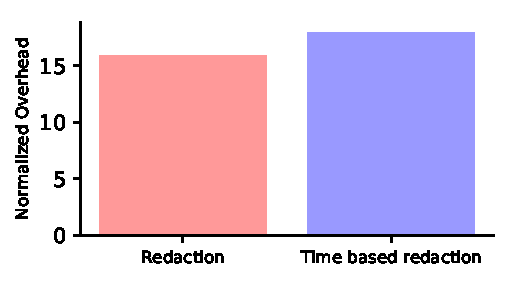
\includegraphics[width=8cm,height=4cm]{fig/policy_latencies.pdf}  
%%   \caption{Normalized latency of servicing an \texttt{open} for different policies with respect to the latency to service a null-policy capsule open request. }
%%   \label{fig:policy_latency}
%% \end{figure}
% %%%%%%%%%%%%%%%%%%%%%/


%% To identify the impact on applications operating on trusted capsules,
%% we look back and reference the work we had done for the first
%% generation prototype. Our experiences when creating the first
%% generation of the prototype have been our guiding principle for making
%% the system perform better. We present here the perceived latencies for
%% applications that operate on capsules while performing some
%% non-trivial tasks. \footnote{The reader is reminded that the following
%%   results are based on the first generation prototype which is based
%%   on the older system that used system call interceptor mechanism as
%%   described in ~\ref{sub:proto-prototype}}

%% We measured the impact under three different conditions: with an empty
%% null policy, with our use case policies, and without trusted capsules
%% (as a baseline). Some of our use case policies, such as those on the
%% PDF and JPEG, required a trusted capsule server in order to fetch
%% remote state and report logged information. For all data type
%% use-cases, we implemented use-case policies described in
%% Section~\ref{sec:new-policies}, except for redactions on PDF
%% documents, which required knowing PDF's binary format.

%% We used a Canon Rebel II DSLR to film certain interactions between the trusted capsule and applications. We then measured the latency between
%% the start of an action (e.g. open a document) and when the action is
%% completed. We filmed at 60 FPS and used the difference in timestamps
%% to calculate the application latency. We present our results in
%% Table~\ref{Tbl-Macro-performance} and provide the raw footage online:
%% \url{https://goo.gl/SiBEJB}.

%%%%%%%%%%



% We used Linaro OP-TEE OS (version 3.3) We modified the Linaro OP-TEE OS version
% 3.3 to be our TrustZone software stack and mounted a userspace filesystem in the
% normal world operating system that runs a custom Hikey Debian OS based on Linux
% kernel 4.4.15. \pu{check} In the FUSE filesystem, we intercept \textit{open} and
% \textit{close} system calls and redirect them to the secure world for decryption
% and encryption respectively. All accesses to non-capsule files proceed just like
% normal file operations on a FUSE mountpoint.

%We deployed ARM Trusted Firmware and a modified Linaro OP-TEE OS as our
%software stack in TrustZone.


%Our trusted capsule monitor in the normal world 
%consists of a modified Linaro OP-TEE supplicant and a modified Linaro OP-TEE Linux 
%Driver with our custom system call interceptor. The kernel components are deployed as
%Linux kernel module. 

% Our modifications to the OP-TEE OS in the secure world is limited to the
% implementation of a few missing \texttt{libc} functions like \texttt{atoi} and
% \texttt{strcmp}. These are minimal changes compared to the original OP-TEE code
% base.

%Our modifications to the OP-TEE components across the
%software stack in both worlds consist entirely of additional RPCs that 
%enable trusted capsule applications to access the file system and network
%directly. These modifications are minimal compared to the original OP-TEE
%code base. % Our implementation is based on OP-TEE 1.0. 


% twithin the OP-TEE Linux Driver that returns predefined longitude and latitude
% values.
%
% In the normal world, we run a pre-alpha release of a custom HiKey Debian OS
% based on Linux kernel 3.18.0.
%
% We used 128-bit AES and SHA-256 for encrypting and hashing trusted
% capsules.

% Our current implementation supports the following composable actions
% based on policy evaluation:

% \begin{itemize}

% \item Allowing or denying the operation on the trusted capsule.

% \item Initializing or modifying persistent state (e.g., counter).

% \item Performing byte-based or keyword-based redaction that partially
%   discloses trusted capsule data. %A data-type specific pre-processor
%   %can be used to generate the byte offsets.

% \item Reporting the operation, location, time, role-identity of the
%   device to a global policy coordinator.

% \item Hard access revocation by deleting the capsule, triggered
%   locally or remotely; and, soft revocation by arbitrarily changing
%   the policy.

% \item Prevent declassification through the network or file system.
% \pu{Review.}


%\item Registering a callback -- to place a deterministic real-time bound on when a policy is re-evaluated 
%\item Killing a running process 

%\end{itemize}

% In total, our trusted capsule application has 4.2K lines of
% non-comment C code and our filesystem code has 2K lines of
% non-comment C code.
 %-- paper (full)
%%%%%%%%%%%%%%%%%%%%%%%%%%%%%%%%%%%%%%%%%%%%%%%%%%%%%%%%%%%%%%%%%%%%%%%%%%%%%%%%
\chapter{Evaluation}
\label{sec:eval}
%%%%%%%%%%%%%%%%%%%%%%%%%%%%%%%%%%%%%%%%%%%%%%%%%%%%%%%%%%%%%%%%%%%%%%%%%%%%%%%%

We evaluated four aspects of our system: \textbf{(1)} the utility and
simplicity of the policy language, %\textbf{(2)} the storage overhead of trusted capsules, 
\textbf{(2)} latency at the system call layer,
and \textbf{(3)} the overhead associated with different policies. %perceived latency at the application layer.

All performance evaluations were performed on our HiKey development board. 
%For the evaluation we used real file types %and applications,
% including JPEG/GpicView image viewer, TXT/Leafpad, and PDF/Evince PDF reader.

%% To interact with these data types, we used GpicView as our image
%% editor, VLC as our video player, LibreOffice writer as our document
%% editor and Evince as our PDF reader.
 
%%%%%%%%%%%%%%%%%%%%%%%%%%%%%%
\section{Policy language}
%%%%%%%%%%%%%%%%%%%%%%%%%%%%%%

In our policy language evaluation we aimed to answer two questions: is
the policy language adequate for expressing useful policies? And, are
these policies easy to express?

We answered our first question by writing trusted capsule policies for
the example use-cases from Section~\ref{sec:new-policies}. For our second
question, we measured the LOC for each policy that we wrote and show
the result in Table~\ref{policy-loc}.

The ability to easily express complex policies tersely is important
both as a proxy of simplicity and to bound the memory overhead of the
Lua interpreter in the secure world. We found that with a few lines of
code we were to express complex policies such as redaction and
revocation.

% We focus on two such policies. The first policy is used in the context
% of a sensitive merger document. We highlight one component of the
% policy, the system-level redaction policy in
% Figure~\ref{fig:merger_policy}.  This policy redacts all data within
% the byte offsets specified by \textit{redact\_sensitive}. These byte
% offsets were translated by a policy pre-processor from
% \textit{$<Sensitive>$} XML-like tags used to define the merger
% document. This redaction only occurs if the document is opened outside
% of the office as determined by the GPS coordinates.  The original data
% is replaced with the character defined by \textit{replace\_char}.

% We show the results in Figure~\ref{fig:redaction}.

%%%%%%%%%%%%%%%%%%%%%
%% \begin{figure}
%%   \centering
%%   \begin{subfigure}{\columnwidth}
%%   	\includegraphics[width=8cm, height=4cm]{../Images/non_redact.jpg}
%% 	\caption{Unredacted merger document.}
%% 	\label{fig:unredacted}
%%   \end{subfigure}\hfill
%%   \begin{subfigure}{\columnwidth}
%%   	\includegraphics[width=8cm, height=4cm]{../Images/redact.jpg}
%% 	\caption{Redacted merger document.}
%% 	\label{fig:redacted}
%%   \end{subfigure}\hfill 
%%   \caption{Before vs. after redaction.}
%%   \label{fig:redaction}
%%   % \vspace{-1em}
%% \end{figure}
%%%%%%%%%%%%%%%%%%%%%/

% The second policy is for photos stored in the cloud. The policy, shown
% in Figure~\ref{fig:image_policy}, allows only devices provisioned
% with the role-based identity ``Kate'' to access the photo. As described
% previously, with trusted capsules, an attacker who gains access to
% photos will not be able to access the capsule contents. On every
% \textit{open} system call, the monitor checks with the policy
% coordinator for updates to a remote state (line 7 in
% Figure~\ref{fig:image_policy}). If the remote server returns
% \textit{true}, the photo is deleted from the device.

% For these and other policies we found that the Lua policy interpreter
% needed less than 2KB of allocated memory.

%% However, while writing our trusted capsule policies, we discovered
%% some gaps in usability. For example, our Lua policy understands time
%% as an integer since January 1, 1970. Converting dates to such an
%% integer may be confusing and awkward. Currently we are exploring a
%% more feature-rich policy processor that would translate between more
%% human-friendly policy inputs to our Lua policy, however this is
%% outside the scope of the current work.

%%%%%%%%%%%%%%%%%%%%%%%%%%%%%%%%%
\begin{table}[h!]
\centering
{\small
\begin{tabular}{|l|c|}
\hline
\textbf{Policy}          & \textbf{LOC} \\ \hline\hline
Location Based Access & 30  \\ \hline
% Location Based Redaction (Using Lua String funcs)    & 63  \\ \hline
Location Based Redaction    & 45  \\ \hline
Content Distribution     & 28  \\ \hline
\end{tabular}
}
\caption{LOC for example policies from Section~\ref{sec:new-policies}.}
\label{policy-loc}
\end{table}
%%%%%%%%%%%%%%%%%%%%%%%%%%%%%%%%%

% TODO Have it import the file from a code directory.
% \begin{figure}
% \begin{lstlisting}[basicstyle=\tiny,linewidth=\columnwidth,xleftmargin=0.1\columnwidth,tabsize=2,numbers=left,breaklines=true,language={Python}]

% %\begin{lstlisting}%[caption={Sensitive Merger Document Policy.}]
% ...
% replace_char = "#"
% redact_sensitive = {45379, 45393, 45532, 45549, 45705, 45726, 45880, 45905, 46081, 46094, 46178, 46185, 46293, 46309, 46380, 46385, 46449, 46458, 46528, 46533, 46606, 46609, 46676, 46682, 46768, 46769, 46835, 46844, 46953, 46963, 47124, 47141, 47225, 47235, 47343, 47348, 47419, 47427, 47491, 47496, 47571, 47586, 47659, 47662, 47729, 47735, 47821, 47822, 47888, 47897, 48006, 48018, 48682, 48684, 48751, 48757, 48843, 48847, 49003, 49008, 49705, 49715, 49926, 49928, 50077, 50079, 50136, 50139, 50950, 50957, 51078, 51080, 51266, 51268, 51325, 51328, 52810, 52823, 54542, 54559};
% redact = {};
% ...
% -- READ
% elseif op == 1 then
% 	local long, lat = getgps();
% 	if((lat - 2130 >= 10) or (2130 - lat >= 10)) or ((lat - 22223 >= 10) or (22223-lat >= 10 )) then
% 		redact = redact_sensitive;
% 	end
% ...
% \end{lstlisting}
% \caption{Sensitive merger document policy.}
% \label{fig:merger_policy}
% \end{figure}

% \begin{figure}
% \begin{lstlisting}[basicstyle=\tiny,linewidth=\columnwidth,xleftmargin=0.1\columnwidth,tabsize=2,numbers=left,breaklines=true,language={Python}]

% %\begin{lstlisting}[caption={Private Image Policy},language={Python},breaklines=true,linewidth=\columnwidth]
% ...
% if getlocalstate( "cred" ) ~= "kate" then
% 	res = false;
% end
% -- OPEN
% if op == 0 then
% 	view_status == getserverstate( "delete?" );
% 	if ( view_status == "true" ) then
% 		delete();
% 	end
% ...
% \end{lstlisting}
% \caption{Private image policy.}
% \label{fig:image_policy}
% \end{figure} 


% %%%%%%%%%%%%%%%%%%%%%%%%%%%%%%
% \subsection{Storage overhead}
% %%%%%%%%%%%%%%%%%%%%%%%%%%%%%%

% Converting regular data into trusted capsules incurs storage overhead
% that is proportional with the policy size. We evaluate
% the associated overhead for different types of data.

% %%%%%%%%%%%%%%%%%%%%%%%%%%%%%%%%%%%%%%%%%%%%
% \begin{table}
% \begin{center}
% {\small
% \begin{tabular}{|l||*{3}{r|}}\hline
% %\backslashbox{Privilege}{World}
% &\makebox{\textbf{Data (KB)}}&\makebox{\textbf{Capsule (KB)}}&\makebox{\textbf{Overhead}}\\\hline\hline
% PDF Doc&137.34KB&139.38KB&1.42\%\\\hline
% JPEG Image&204.10KB&207.00KB&1.42\%\\\hline
% MP4 Video&4142.40KB&4175.94KB&0.80\%\\\hline
% LibreOffice Doc&54.80KB&56.70KB&3.47\%\\\hline
% \end{tabular}
% }
% \caption{Storage overhead for test data files.}
% \label{Tbl-StorageOverhead}
% \end{center} 
% \end{table}
% %%%%%%%%%%%%%%%%%%%%%%%%%%%%%%%%%%%%%%%%%%%%

% Table~\ref{Tbl-StorageOverhead} lists the storage overhead for a PDF,
% JPEG, MP4, and FODT files used in our evaluation. These data types were
% converted to trusted capsules with 4KB chunk sizes. We found the
% storage overhead to be negligible.

%%%%%%%%%%%%%%
\section{System call microbenchmarks}
%%%%%%%%%%%%%%


\begin{figure}[t]
  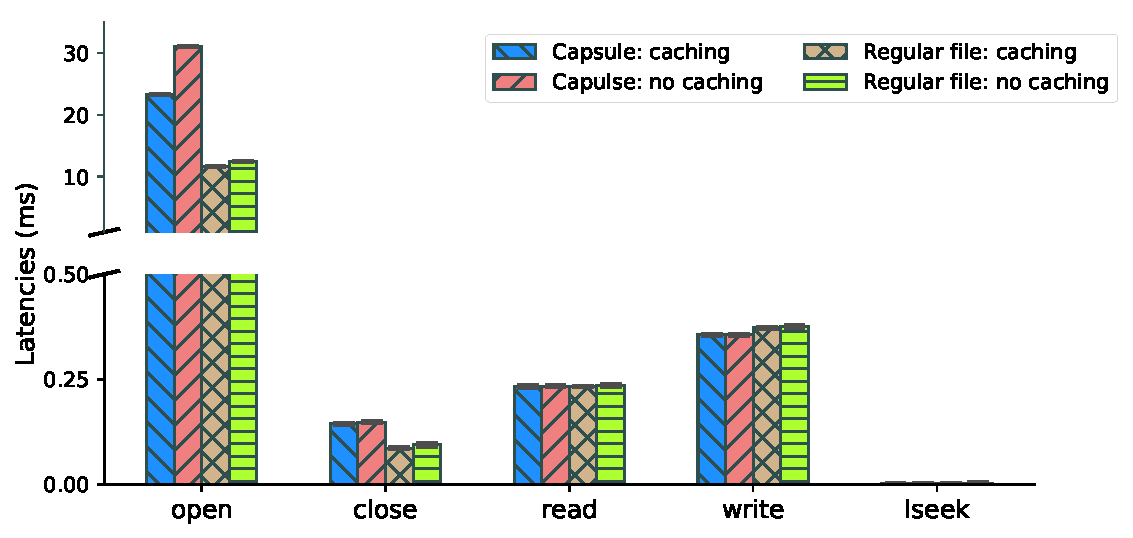
\includegraphics[width=8cm,height=4cm]{fig/latencies.pdf}
  \caption{Average system call latency}
  \label{fig:latencies}
\end{figure}

\begin{figure}[t]
  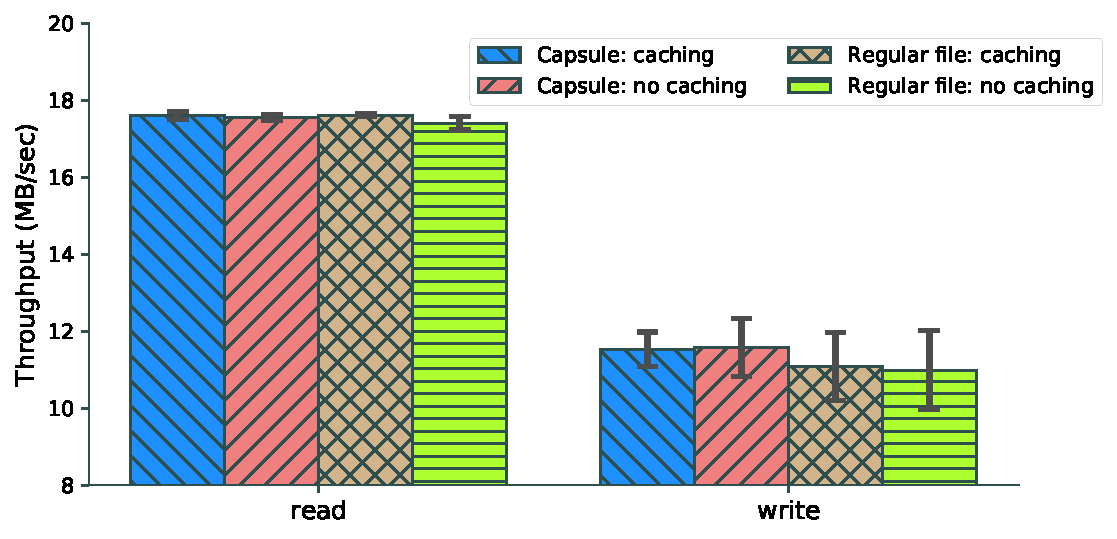
\includegraphics[width=8cm,height=4cm]{fig/rw_throughput.pdf}
  \caption{Throughput of Read and Write operations to a capsule}
  \label{fig:rw_throughput}
\end{figure}


In considering system call level microbenchmarks, we focus on three
questions.\\

\textbf{Are operations on regular files affected?} 
We measured the latency of filesystem operations for a regular file and a capsule. Since our system is based on FUSE, we evaluate the performance of the Trusted Capsule system by comparing against system call latencies for a regular file on the same mountpoint.

% We measured the
% performance of system call operations with and without the system call
% interceptor for both latency and throughput under similar conditions.
%Operations on regular data represents the fast path in our interceptor. 
We found that the performance of system calls on regular data is not impacted, except for \textit{open} syscall. 
This is due to the overhead of checking whether the target file is a trusted capsule. \\
%In addition, once a process
%has accessed a trusted capsule, write throughput on regular data also decreases linearly with
%number of trusted capsule accessed by that process due to the need to evaluate each trusted capsule's 
%declassify policies. 

\textbf{What is the latency and throughput of the system calls we
  intercept for operations on trusted capsules?} We measured the
latency and throughput of syscall operations on trusted capsules.  For
latency measurements, we measured the end-to-end time for a syscall
and averaged over 1000 runs.  For throughput measurements, we randomly
read and wrote 4KB of data to a trusted capsule for 10 seconds. To get an estimate of performance on the first use, we repeat the experiment with a cold cache achieved by dropping the page cache. 
For each test trusted capsule, we attached an empty null policy that always evaluated to true.  We present our results in Figure~\ref{fig:latencies} and ~\ref{fig:rw_throughput}.

The latency for \texttt{open} and \texttt{close} operations for a capsule present a prominent spike when compared to the operations on regular files. This is expected since our current prototype interposes on only these operations. An \texttt{open} operation on a null-policy capsule (warm cache) completes in 23 milliseconds compared to the 11.7 milliseconds for a regular file. The close operation on a capsule completes in  144 microseconds as compared to  86 microseconds for a regular file. 

The observed altency spike is more pronounced for \texttt{open} than for \texttt{close}. We understand this to be a direct result of the greater number of steps that have to happen in TrustZone to initialize the Trusted Application, which do not need to be done  while servicing a capsule close. 

We were able to achieve 17.59MB/s throughput for reading and 11.52MB/s throughput for writing to a no-op capsule on a warm cache. This is comparable to the read (17.6 MB/s) and write throughput (11.1 MB/s) achieved for a regular file when accessed in the same experimental setup. When the same experiments were repeated for a cold cache, the throughput drops marginally.

The read and write throughputs for a capsule, as compared to a normal
file, were expected to be nearly identical. This is expected in our
system since all reads and writes to a capsule gets directed to a
shadow file, which is treated like a regular file in FUSE.


% While we initially expected some impact to read and write performance at smaller chunk sizes, our
% results showed otherwise. We believe this may be due the fact that the cost of extra round trips between
% normal and secure world to fetch the same quantity of data is not significant overall.
% We also incur significant costs for \textit{open} syscall, especially at larger file sizes. 
% %Again, chunk size has little impact on performance. 
% While we do not expect \textit{open} syscall to be called often by applications 
% that interact with trusted capsule, its poor performance nevertheless requires further optimization. In our 
% current implementation, an \textit{open} syscall makes a pass over the entire data of the trusted capsule
% to validate the trusted capsule contents against its hash. This results in longer latencies as the file size
% increases. As can be seen, we were able to obtain reasonable results for \textit{open} calls on file sizes that
% were less than 100KB. However this latency increases dramatically for larger file sizes. 
% %In the future, we plan to explore possible optimizations. 


%For throughput, 
%we use 4KB request sizes as this is the granularity that most applications 
%read/write~\cite{evalpaper,filenotafile}. The throughput was run over a 10 second period.

%\begin{figure}[h!]
%	\includegraphics{../Graphs/Microbenchmarks_Latency.pdf}
%	\caption{The average latency per operation on a regular 1M file in varying system state (load and interceptor) with 95\% error bars.}
%	\label{micro_latency}
%\end{figure}

%\begin{figure}[h!]
%	\includegraphics{../Graphs/Microbenchmarks_Throughput.pdf}
%	\caption{The throughput measured over a ten second period on a regular 1M file in varying system state (load and interceptor).}
%	\label{micro_throughput}
%\end{figure}

% %%%%%%%%%%%%%%%%%%%%%
% \begin{figure}
%   \centering
%   \begin{subfigure}{\columnwidth}
%   	\includegraphics[width=8cm, height=4cm]{../Graphs/Chunk_Size_Comparison_Latency.pdf}
% 	\caption{Average latency varied by chunk size. The bars represent 95\%.}
% 	\label{fig:chunksize_latency}
%   \end{subfigure}\hfill
%   \begin{subfigure}{\columnwidth}
%   	\includegraphics[width=8cm, height=4cm]{../Graphs/Chunk_Size_Comparison_Throughput.pdf}
% 	\caption{Throughput varied by chunk size.}
% 	\label{fig:chunksize_throughput}
%   \end{subfigure}\hfill 
%   \caption{System call performance varied by chunk size. Test trusted capsules had a data size of 1M.}
%   \label{fig:chunksize}
%   % \vspace{-1em}
% \end{figure}
% %%%%%%%%%%%%%%%%%%%%%/

% %%%%%%%%%%%%%%%%%%%%%
% \begin{figure}
%   \centering
%   \begin{subfigure}{\columnwidth}
%   	\includegraphics[width=8cm, height=4cm]{../Graphs/File_Size_Comparison_Latency.pdf}
% 	\caption{Average latency varied by file size. The bars represent 95\%.}
% 	\label{fig:filesize_latency}
%   \end{subfigure}\hfill
%   \begin{subfigure}{\columnwidth}
% 	\includegraphics[width=8cm, height=4cm]{../Graphs/File_Size_Comparison_Throughput.pdf}
% 	\caption{Throughput varied by file size.}
% 	\label{fig:filesize_throughput}
%   \end{subfigure}\hfill 
%   \caption{System call performance varied by file size. Test trusted capsules created using 4KB chunk size.}
%   \label{fig:filesize}
%   % \vspace{-1em}
% \end{figure}
% %%%%%%%%%%%%%%%%%%%%%/

%\textbf{Tainted Processes.} \ac{Add better explanation of what this is showing.} We start the a 
%process. It sequentially opens each of our 
%use case capsules. Then we call write() on a regular file with 4KB request sizes at random
%offsets 10000 times. 

%Opened three different capsules with no-op policies: \ac{file size/chunk size per capsule here}.

%We see large degradation of the read throughput based on the number of capsules open. The write %throughput with no capsules open is about 2.0 MB/sec, once one capsule is open, the throughput drops to %0.5 MB/sec. 

% \begin{figure}[h!]
% 	\includegraphics{../Graphs/Tainted_Process.pdf}
% 	\caption{The throughput cost of having multiple capsules open while accessing a regular file.}
% 	\label{tainted_process}
% \end{figure}

% \textbf{What is the contribution of various aspects of the trusted
%   capsule monitor to per-operation latency overhead?} We evaluated the
% cost of the (1) normal world data monitor components (interceptor and
% linuxdriver), (2) world switch, (3) hashing, (4) encryption, (5)
% secure storage operations, (6) direct file system operations and (7)
% policy engine initialization.  We average our results over 100
% iterations of the same system call. Our test capsule had an empty null
% policy and used 4KB chunksize and consisted of 1MB of data. We show
% the results for (3)-(7) in
% Figure~\ref{fig:1M_4KB_breakdown_cycles}. We measured costs of these
% components end-to-end. For example, a secure storage operation in
% Figure~\ref{fig:1M_4KB_breakdown_cycles} would include the cost of
% world switches, userspace and kernel space boundary crossings, copying
% data between layers of the software stack and RPCs. All measurements
% are based on a 1.2 MHz monotonic counter.

% We found accessing secure storage to be an extremely expensive operation, accounting for a large number of cycles. This occurs when 
% policy evaluation needs to access state and on instantiation of the trusted capsule session when the cryptographic information is fetched.
% Further, the moderate costs associated with direct file system operations is in-line with
% our observation that decreasing chunk size (increasing the number of direct file system operations) did not affect performance 
% extensively. Surprisingly, encryption and hashing was not as a significant component of the overall cost as we thought. 
% Further, initializing the Lua interpreter, the normal world data monitor components (interceptor and
% linuxdriver) and world switching represented marginal costs. We measured the cost of both the normal world data monitor components and 
% evaluated the null policy to be few dozen cycles and a world switch to cost only a single cycle. 

% Perhaps the most interesting observation is that all these aspects (1)
% to (7) combined accounted for only $\sim$30\% of total cost of any
% syscall operation. These operations represent all the transitions that
% may occur between the trusted application and the remainder of the
% software stack (normal world components, OP-TEE OS, etc.), except for
% memory allocations (both between secure and normal world, and between
% userspace and kernel space within the secure world) and trusted
% application code. This leads us to believe that a significant portion
% of the slowdown is due to memory management across the stack and the
% in-memory copies and loops in the trusted application.

% To further evaluate the impact of world switch overhead, we measured the number of world switches for each operation. We broken down the
% world switch for different purposes. For any operation, we found that it required at most $\sim$100 world switches at a cost of 1-2 cycles per
% world switch. We make an interesting observation that most world switches are used to handle RPCs and their associate shared memory 
% allocations. 

% %%%%%%%%%%%%%%%%%%%%%
% \begin{figure}
%   \centering
%    \begin{subfigure}{\columnwidth}
%     \includegraphics[width=8cm, height=4cm]{../Graphs/Counter_Cycles_Breakdown_test_1M_NULL_4KB.pdf}
% 	\caption{Operations.}
% 	\label{fig:1M_4KB_breakdown_cycles}
%   \end{subfigure}\hfill 
%   \begin{subfigure}{\columnwidth}
%   	\includegraphics[width=8cm, height=4cm]{../Graphs/World_Switches_Breakdown_test_1M_NULL_4KB.pdf}
% 	  \caption{World Switches.}
% 	\label{fig:1M_4KB_breakdown_switches}
%   \end{subfigure}\hfill
%   \caption{Breakdown of number of cycles spent performing specific operations and number of world switches for specific purpose.}
%   \label{fig:1M_4KB_breakdown}  
%   % \vspace{-1em}
% \end{figure}
% %%%%%%%%%%%%%%%%%%%%%/

% \begin{figure}[h!]
	
% \end{figure}

% \begin{figure}[h!]
	
% \end{figure}

\section{Policy Performance Evaluation}

% We evaluate the performance of our trusted capsules at the macro-level
% directly with unmodified applications. We investigated how the
% overhead incurred by trusted capsules at the system call level impacts
% performance at the application level. For this purpose we used our use
% case trusted capsules.

In this section we present our preliminary findings on the impact that
policies of varying complexity have on the performance of the
system. %% We also present our past experience with making the older
%% system work with unmodified applications and the impact on the
%% perceived application slowdown.

To measure the overhead associated with the policy execution, we
compare the latency microbenchmarks for \texttt{open} operations for a
policy containing capsule, normalized with respect to the latency for
opening a null-policy capsule. These results are presented in
Figure~\ref{fig:policy_latency}. There is a sharp increase in the
latency when there is a non-null policy being evaluated, and this
latency increases with the complexity of the policy.

Figure~\ref{fig:policy_latency} compares two policies: a redaction
policy that redacts sensitive tags without performing other checks and
a local time based redaction policy, which performs redaction based on
the epoch value obtained from the device. The redaction policy uses
the \texttt{redact()} API from Table~\ref{Tbl:lua_ext}, while the Time
based redact policy uses the \texttt{redact()} API as well as well as
the \texttt{getTime()} API. This extra work to service an open request
is evident from Figure~\ref{fig:policy_latency}.

%%%%%%%%%%%%%%%%%%%%%%%%%%%%%%%%%%%%%%%%%%%%%%%%%%%%%%%%
\begin{figure}[t]
    \centering
    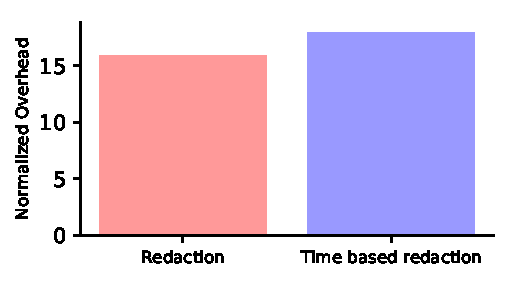
\includegraphics[width=8cm,height=4cm]{fig/policy_latencies.pdf}
    \caption{Normalized latency of servicing an \texttt{open} for different policies with respect to the latency to service a null-policy capsule open request. }
    \label{fig:policy_latency}
\end{figure}
%%%%%%%%%%%%%%%%%%%%%%%%%%%%%%%%%%%%%%%%%%%%%%%%%%%%%%%%


%% \begin{table*}[t]
%% \begin{center}
%% {\small
%% \begin{tabular}{|l|l|l|*{3}{r|}}\hline
%% %\backslashbox{Privilege}{World}
%% \makebox{\textbf{Data Type}}&\makebox{\textbf{Application}}&\makebox{\textbf{Interactions}}&\makebox{\textbf{Regular Data}}&\makebox{\textbf{Null Policy}}&\makebox{\textbf{Use-Case Policy}}\\\hline\hline
%% PDF Doc&Evince&Open document&0.87s&3.20s&110.40s\\\hline
%% JPEG Image&Gpicview&Open image, rotate, save&0.45s/0.23s/0.17s&6.45s/0.88s/3.43s&20.23s/1.43s/11.38s\\\hline
%% MP4 Video&VLC&Buffering time before playing&3.21s&3.92s&25.72s\\\hline
%% LibreOffice Doc&LibreOffice Writer&Open document&1.63s&12.42s&21.67s\\\hline
%% \end{tabular}
%% }
%% \caption{Application level performance as observed from first prototype's evaluation}
%% \label{Tbl-Macro-performance}
%% \end{center} 
%% \end{table*}


%%  We believe that such performance degradations can be
%% mitigated with more efficient policy code, for example policies that
%% run at coarser granularity or use caching to mitigate expensive
%% checks.
 %-- paper (abridged)
\chapter{Limitations}
\label{sec:limitations}

Now we turn to discuss the design limitations of Trusted Capsules. In this
section we cover the limitations imposed by our design choices and the
limitations imposed by the specific choice of software and hardware. Moreover,
we take a gander at why Trusted Capsules remains a rather naive attempt at
solving the problem of retrofitting existing applications with security
extensions.

\subsection{Desgin Limitations}
\begin{enumerate}
    \item {\bf Inability to limit trust in optimistic state}: In the optimistic state, we
trust the normal world kernel, the app, and the user, to not leak capsule data
to unauthorized apps. Such trust may not be warranted even in a non-adversarial
setting. For example, an app might create temporary copies of the files it has
opened into a world-readable directory or the user might copy the data into the
system clipboard. While we may use techniques such as information flow control
to detect such data leaks, doing so would prohibitively impact performance.

    \item {\bf Lack of app semantics}: Since we interpose only on the {\tt open()} and
    {\tt close()} syscalls to execute policies, a policy may not reason about {\em
        why} an app is opening a file. For example, when a user opens a document in a
text editor, it may open the file multiple times to seek through the file in
parallel. Hence, while the capsule was opened just once from a user's
perspective, the policy would observe multiple capsule access attempts. Policies
that rely on access logs have to be aware of this disconnect.

    \item {\bf Abusive policies}: Although we run capsule policies in a sandbox, we do not
completely prevent all damages a malicious policy can inflict. It can, for
example, access a user's GPS data and send them to a server for the purpose of
tracking her whereabouts. To handle this limitation, we either need some
systematic way of vetting the data a policy sends to a remote server or prevent
it from sending device data altogether.
\end{enumerate}

%%%%%%%%%%%%%%%%%%%%%%%%%%%%%%%%%%%%%%%%%%%%%%%%%%%%%%%%
\begin{figure}[t]
    \centering
    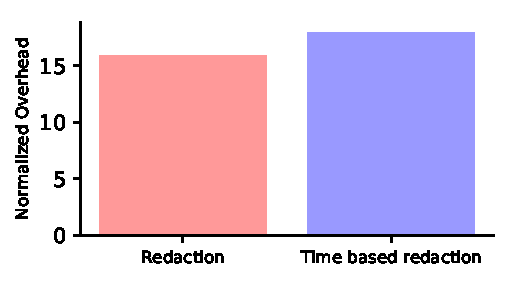
\includegraphics[width=8cm,height=4cm]{fig/policy_latencies.pdf}
    \caption{Normalized latency of servicing an \texttt{open} for different policies with respect to the latency to service a null-policy capsule open request. }
    \label{fig:policy_latency}
\end{figure}
%%%%%%%%%%%%%%%%%%%%%%%%%%%%%%%%%%%%%%%%%%%%%%%%%%%%%%%%


\subsection{Prototype Limitations:}
In this section we list the limitations that bound the current prototype from
realizing the fulll vision of the Trusted Capsule model of data protection.
Here we note some design and implementation limitations.

\begin{enumerate}
    \item FUSE can be used interpose on only the file I/O system calls that are
directed to a FUSE serviced mountpoint. This poses some challenges in making
Trusted Capsules work seamlessly with an unmodified application.\\There is no
way for the FUSE filesystem code to identify when a process that had been
issuing IO to the mountpoint dies. The implication of this fact for the
prototype is that there is no good and atomic way to delete the shadow file on
the termination of the process. The prototype handles this by setting up a
background process that monitors if the process that had accessed the mountpoint
has terminated.
    \item The stock configuration for the TrustZone memory partitions makes the
Secure World a very memory constrained environment. The memory that is available
in the secure world is only 10 MB, and that needs to host the Secure OS as well
as any trusted application code that must run in Trustzone. Linaro OP-TEE
recently included dynamic shared memory in their Secure OS, but to access those
features, one has to have a higher kernel version than what gets shipped with
the stock Debian OS rootfs image. Higher Linux kernel versions have known
problems with the HDMI drivers, which causes the Linux kernel to panic when a
monitor is plugged in.
    \item This limitation hits our prototype particularly badly. In the
current prototype, we send a copy of the entire file to TrustZone to decrypt.
Since there are severe restrictions on the amount of memory available in
TrustZone, we are unwittingly bounded on the maximum file size that can be
processed as a capsule.
    \item The implementation has a limitation that it
needs to create copies of the data buffers to process each part of the capsule.
This creates more memory pressure in an already resource constrained
environment. 
\end{enumerate}


%%%%%%%%%%%%%%%%%%%%%%%%%%%%%%%%%%%%%%%%%%%%%%%%%%%%%%%%%%%%%%%%%%%%%%%%%%%%%%%%
\chapter{Related Work}
\label{sec:related}
%%%%%%%%%%%%%%%%%%%%%%%%%%%%%%%%%%%%%%%%%%%%%%%%%%%%%%%%%%%%%%%%%%%%%%%%%%%%%%%%

\textbf{Securing data with policies}: The concept of associating policies to
data to authenticate accesses to that data is not new. An early expression of
this is XACL, which specifies access control policies within XML
documents~\cite{xacl}. Karjoth et al. proposed using {\em sticky policies} to
provide enterprises better oversight over the customer data they
collect~\cite{karjoth02enterprise}. These policies capture customer-specified
requirements (e.g.: ``delete my data after 30 days'') and are associated with
the collected data. They are then enforced cooperatively within the enterprise
as the data is used. Subsequent work strengthened this scheme by encrypting the
data bundled with the policy using IBE (identifier-based encryption) and
decrypting it only if its policies are satisfied~\cite{mont03stickypolicies,
  pearson11stickypolicies}. Encrypting the data reduces the need for cooperation
and allows sharing data across enterprise boundaries

Maniatis et al. outlined a vision that allows {\em all} users to protect their
data before they share them across machine boundaries~\cite{datacapsules}. Their
conceptual architecture uses the sticky policy approach to package data in units
known as {\em data capsules}. When an application needs to use a capsule and
satisfies the capsule's policies, an abstract secure execution environment
decrypts the capsule and executes the application. An implementation of this
architecture was left as an open question.

More recent works use trusted computing features on mobile devices to protect
data with the sticky policy approach. Li et al. proposed DroidVault to allow
employees in an enterprise to securely store and process sensitive company data
on their untrusted Android devices~\cite{li14droidvault}. Its architecture only
allows trusted code signed by the enterprise to operate on the data and executes
it in ARM TrustZone.  To display data and receive user inputs, it relies on
secure I/O between the peripherals (display, keypad, etc.) and TrustZone. This
architecture ensures unencrypted versions of the sensitive data do not leave the
TrustZone environment. Lazouski et al. proposed using TPMs (Trusted Platform
Modules) to ensure only vetted versions of the OS and applications are loaded
before accessing sensitive data and executing their
policies~\cite{lazouski14stateful}. In principle, this approach allows policy
execution and data access in normal world (outside TrustZone) while guaranteeing
the absence of malicious applications.

Other related work in this area include Excalibur, which enables a cloud
provider to protect data stored in its cloud from being exfiltrated by its
administrators who have access to the cloud management
interface~\cite{excalibur}; PCD (policy-carrying data), which lets an end user
attach terms of service to his data before sharing it cloud service providers
and thereby disincentivizing them from misusing the data ~\cite{policydata};
Ryoan, which enables users to submit their sensitive data to a cloud service
provider for processing without requiring either the user to disclose the data
or for the provider to release their proprietary code~\cite{ryoan}; and P3, a
private photo-sharing service that protects images shared by users from
untrusted service providers~\cite{p3}.

Trusted Capsules differs from these in its aim and scope: it uses the sticky
policy technique to allow end users to protect their own data as they share it
with other end users and unlike P3, it is data type agnostic. While Trusted
Capsules uses ARM TrustZone to securely execute the policies, it allows unvetted
normal world processes to access unencrypted sensitive data in the optimistic
state (unlike DroidVault and the work by Lazouski et al.). Our approach is
motivated by usability concerns as we want authorized users to be able to use
their desired third-party apps to process sensitive data.

There are now startups that have emerged as players in the domain of providing data security systems. A startup called Sandstorm ~\cite{sandstorm} abstracts data 
as a \textit{grain} -- a package of all 
the apps, libraries, and configuration files needed to operate on a single 
piece of data locally within a container. Sandstorm then creates an 
enclosure around the container and interposes on all operations to enforce the \textit{grain}'s
access policies.
Unlike trusted capsules, which operates at the granularity of a
piece of data, Sandstorm operate at the granularity of an entire
software ecosystem for the data.

\textbf{Information Flow Control based mechanisms}: There has also been a vast body of research that studies providing data confidentiality through label-based solutions such as Distributed Information Flow Control ~\cite{jif, asbestos, histar, dstar, laminar, aeolus, flume}. They use labels to specify access control, 
capabilities, and authority. These labels are used to track the flow of information at various levels of the software stack. 

By not allowing data to move to processes that 
do not have the right labels, DIFC prevents sensitive data from being exfiltrated. 
 
In DIFC, labels create a natural ecosystem for composition that allow a process to access multiple pieces of data. Trusted capsules are less composable. 
If two trusted capsules have contradictory policies, they
cannot be accessed by a process at the same time. On the other hand, trusted capsules are backward compatible 
and do not require constructing a complex security lattice as in DIFC.

Another popular approach is tainting~\cite{demandemulation, neon,
taintdroid, practicaltainting}. It tracks information flow by interposing
on the system operations at the instruction-level. 
%In this way, such a
These solution can track the flow of information at extremely fine
granularity. %without changes to the application or operating system. 
However they are resource intensive, both in memory
and CPU. 

\textbf{Policy Based Isolation Mechanisms}: Traditional isolation-based solutions remain one of the most widely used practical solutions currently to provide data protection. These solutions, such as VPN, VMWare Ace~\cite{VMWareAce}, Secure Spaces~\cite{securespaces} and Hypori~\cite{hypori}, attempt to prevent
sensitive data from leaving in the first place by enforcing policy at
the network boundary between external and internal systems. 
In these cases, policies that restrict movement of sensitive data can still be
defeated by transformations, such as encryption and compression.
In addition, some of these solutions incur substantial network cost as they do not support offline operations. 

Finally, other work has sought to ensure data confidentiality by
enforcing application structures~\cite{Cleanroom, privacycapsules},
limiting data lifetimes~\cite{enforcinglifetime, lacuna} and providing
recourse actions such as backtracing intrusions~\cite{Backtracking, taser}.


\textbf{Other TEE work}: The research community has used TEEs such as ARM
TrustZone and Intel SGX for a variety of purposes - to provide a secure environment for running VMs, secure partitions or executing parts of third-party applications and to store their data   ~\cite{TLR, Nokia1, Nokia2}, to provide a root-of-trust for performing runtime measurements ~\cite{restrictedspaces, hypervision,SKEE,secvisor} and to secure peripherals ~\cite{TrustedSensors}. In general, these are
orthogonal to Trusted Capsules. 

VButton uses TrustZone to attest whether the UI
inputs on the smartphone were initiated by the user~\cite{li18vbutton}; SeCloak
provides direct control (on/off) over device peripherals even when the normal
world OS is compromised~\cite{lentz18secloak}; Truz-Droid enables users to
securely input and send secrets e.g., login credentials, to authorized servers
without executing third-party code in TrustZone~\cite{ying18truzdroid};
TrustShadow protects applications from untrusted OSes by executing them with a
runtime in TrustZone~\cite{guan17trustshadow}; and SchrodinText allows the
untrusted normal world OS to render sensitive text in the display received from
an application backend server without revealing the contents of the
text~\cite{sani17schrodintext}; DelegaTEE, which uses Intel SGX to enable users
to share their access to online service providers without revealing their
credentials~\cite{matetic18delegatee}.


%%%%%%%%%%%%%%%%%%%%%%%%%%%%%%%%%%%%%%%%%%%%%%%%%%%%%%%%%%%%%%%%%%%%%%%%%%%%%%%%
\chapter{Conclusion}
\label{sec:conc}
%%%%%%%%%%%%%%%%%%%%%%%%%%%%%%%%%%%%%%%%%%%%%%%%%%%%%%%%%%%%%%%%%%%%%%%%%%%%%%%%

Data security on remote devices that the data owner cannot control
represents a unique challenge in our data promiscuous world.  Systems
exchange data indiscriminately and do not offer the data owner any
ability to control access policy on remote devices. At best, data is
encrypted to prevent declassification. %% But, once the data is
%% distributed, the data can travel without restraint.

We introduced graduated access control and realized it using a trusted
capsule abstraction and a data monitor that runs inside ARM's
TrustZone trusted execution environment. Our solution builds on the
file abstraction and does not require any modification to
applications, is gradually deployable, and can be ported to other
kinds of trusted execution environments.

%% Our evaluation demonstrates that
%% graduated access control
%% latency and throughput overhead is reasonable for existing popular
%% applications like a word processer, video/image viewer, and pdf reader.


%% Our evaluation demonstrates that the graduated access control model is
%% useful for a variety of the joint utility and security requirements of
%% a broad range of classes of day-to-day activities by entities with
%% specific security concerns.

%%  with existing and unmodified applications while enabling the
%% data owner to express advisory policies that act as the minimum data
%% policy across all systems and applications.

%% The trusted capsules abstraction ties policy to data -- offering to our
%% knowledge for the first time a universal policy abstraction. Our realization
%% of this abstraction, relying on ARM's TrustZone, provides the data
%% owner with the fine-grained control over the data and its policy
%% across system boundaries. The owner will be able to monitor data
%% access as it occurs, retroactively change data policy and locally 
%% evaluate access policy based on local and remote state. Its advisory policy 
%% capabilities can satisify the joint utility and security requirements of a 
%% broad range of classes of day-to-day activities by entities with specific security concerns.
 %-- full

%    2. Main body
% Generally recommended to put each chapter into a separate file
%\include{relatedwork}
%\include{model}
%%%%%%%%%%%%%%%%%%%%%%%%%%%%%%%%%%%%%%%%%%%%%%%%%%%%%%%%%%%%%%%%%%%%%%%%%%%%%%%%%
\chapter{Prototype}
\label{sec:implement}
%%%%%%%%%%%%%%%%%%%%%%%%%%%%%%%%%%%%%%%%%%%%%%%%%%%%%%%%%%%%%%%%%%%%%%%%%%%%%%%%

We prototyped Trusted Capsules on a LeMaker HiKey development
board~\cite{hikey}. It has an octa core ARM Cortex-A53 processor, 2~GB
of RAM, 8~GB of flash storage. and it comes with TrustZone unlocked,
thereby allowing us to control what OS runs on the TEE. We use Linaro
OP-TEE OS (version 3.3) in TrustZone and a HiKey Debian OS (based on
Linux 4.4.15) in the normal world. We modified the OP-TEE OS to
implement several missing {\tt libc} functions (such as {\tt atoi} and
{\tt strcmp}). As the HiKey board does not have a GPS receiver, we
mocked a GPS device that returns predefined longitude and latitude
values.

Capsules are encrypted with 128-bit AES. We consider the distribution
of keys required to decrypt capsules outside the scope of this paper.

Our data monitor is written in C and consists of about 6.2K SLOC: the
policy execution engine, which runs within the TEE, has about 4.2K
SLOC while the normal world framework has 2K.

%%%%%%%%%%%%%%%%%%%%%%%%%%%%%%%%%%%%%%%%%%%%%%%%%%%%%%%%%%%%%%%%%%%%%%%%%%%%%%%%%%%%%
\subsection{Prototype Evolution}\label{sub:proto-prototype}
%%%%%%%%%%%%%%%%%%%%%%%%%%%%%%%%%%%%%%%%%%%%%%%%%%%%%%%%%%%%%%%%%%%%%%%%%%%%%%%%%%%%%

The system design and the prototype evaluated in this paper has
evolved from a previous design of the system. This prior system
(``version-0'') had the ambitious goal of evaluating a Lua-based
policy in TEE on all intercepted file I/O system calls on a capsule
file: \texttt{open}, \texttt{close}, \texttt{read}, \texttt{write},
and \texttt{lseek}. As well, Version-0 revealed \emph{chunks} of the
file to normal world applications, rather than decrypting and
revealing the entire file contents on \texttt{open}. Version-0 was not
based on FUSE, but it used a custom system call interceptor in the
normal world OS. This interceptor worked in a manner similar to the
FUSE filesystem in our current design

Version-0 prototype was mature and stable, but had to be abandoned
because of unacceptable application slowdown. This was due to the
invasive nature of the system call handler that slowed down the
behaviour of most applications that open and close many files at
start-up. 

More concretely, the time to open a small document under a no-op
policy with FUSE on our hardware is 24ms, %\iv{.5s}
while the latency in Version-0 was 1.2s. %\iv{5s}. 
This is a speed-up of 50x over Version-0.

%By contrast, in our current prototype the
%latency is \iv{1s}, which is a speed up of \iv{5x} over Version-0. 

The latency and throughput gap dramatically increased for large and
complex file types, such as PDF JPEG. This can be observed in the raw
video footage for several use-cases in Version-0 of the system:
\url{https://goo.gl/SiBEJB}.

We note that while overhead in Version-0 was significantly better at
the application layer as compared to the system call layer,
nevertheless, the cost was prohibitive and was tightly connected to
the policy being used.
%
%% %% For various data types, a null
%% %% policy had much less significant or almost imperceivable impact to
%% %% usability at the application level. However, 
%% our use-case policies, some of which contained expensive policy checks
%% (e.g., access to state storage or going over the network to talk to
%% the policy coordinator) on frequent operations such as read or write,
%% resulted in noticeable performance degradation.
%
For example, our MP4 video played smoothly with a null policy in VLC
(which did not interact with the trusted capsule server), but degraded
to extreme jitter once we added a policy that reported actions to a
policy coordinator and accessed secure storage for every read
operation. This effect was particularly acute for the PDF reader,
which repeatedly read the data in small chunks frequently and even
when the user was idle. Each read by the PDF incurred the cost of a
single round-trip to the trusted capsule server, requiring on average
5ms each. 

Our experiences with Version-0 of the Trusted Capsules prototype have
been our guiding principle in making our current system perform
better.
%
Our benchmarking results (presented in the next Section) indicate that
the current Trusted Capsules design, that evaluates policy exclusively
on \texttt{open} and \texttt{close} calls strikes a better trade-off
between security and performance.


%% Our prototype
%% supports the following composable policy actions:

%% \begin{itemize}

%% %\item Allowing or denying the operation on the trusted capsule.

%% \item Allowing or denying the capsule to be opened or modified based on various
%%   signals such as location, time, or device identity.

%% % \item Reporting the operation, location, time, role-identity of the
%% %   device to a global policy coordinator.

%% \item Logging capsule accesses and reporting them to a remote server.

%% %\item Initializing or modifying persistent state (e.g., counter).

%% \item Initializing or modifying persistent capsule metadata (e.g., counter).

%% % \item Performing byte-based or keyword-based redaction that partially
%% %   discloses trusted capsule data. %A data-type specific pre-processor
%% %   %can be used to generate the byte offsets.

%% \item Performing byte-based or keyword-based redaction that partially discloses
%%   trusted capsule data. \ar{Table~\ref{Tbl:lua_ext} doesn't list the API to
%%     perform keyword-based redaction.} \pu{all redaction is based on byte offsets. the keyword search happens in lua and then the byte offsets are passed to the C API. How should I phrase this then?}

%% \item Hard access revocation by deleting the capsule, triggered
%%   locally or remotely; and, gradual access revocation based on evolving policy decisions that are adaptive to context of access - for example, total number of accesses, passage of time, policy updation, etc.
%%   %soft revocation by arbitrarily changing
%%   %the policy. 
%%   \ar{What's soft revocation?}\pu{Check}

%% % \item Prevent declassification through the network or file system.


%% %\item Registering a callback -- to place a deterministic real-time bound on when a policy is re-evaluated
%% %\item Killing a running process

%% \end{itemize}


%% %%%%%%%%%%%%%%%%%%%%%%%%%%%%%%%%%%%%%%%%%%%%%%%%%%%%%%%%%%%%%%%%%%%%%%%%%%%%%%%%%%%%%
%% \subsection{Prototype Limitations}\label{sub:proto-limitations}
%% %%%%%%%%%%%%%%%%%%%%%%%%%%%%%%%%%%%%%%%%%%%%%%%%%%%%%%%%%%%%%%%%%%%%%%%%%%%%%%%%%%%%%

%% %% In this section we list the limitations that bound the current
%% %% prototype from realizing the fulll vision of the Trusted Capsule model
%% %% of data protection. Here we note some design and implementation
%% %% limitations.

%% FUSE can interpose on only the file I/O system calls that are directed
%% to a FUSE serviced mountpoint. This poses some challenges in making
%% Trusted Capsules work seamlessly with an unmodified application. We assume 

%% There is no way for the FUSE filesystem code to identify when a
%% process that had been issuing IO to the mountpoint dies. The
%% implication of this fact for the prototype is that there is no good
%% and atomic way to delete the shadow file on the termination of the
%% process. The prototype handles this by setting up a background process
%% that monitors if the process that had accessed the mountpoint has
%% terminated.

%% The stock configuration for the TrustZone memory partitions makes the
%% Secure World a very memory constrained environment. The memory that is
%% available in the secure world is only 10 MB, and that needs to host
%% the Secure OS as well as any trusted application code that must run in
%% Trustzone.

%% This limitation hits our prototype particularly badly. In the current
%% prototype, we send a copy of the entire file to TrustZone to
%% decrypt. Since there are severe restrictions on the amount of memory
%% available in TrustZone, we are unwittingly bounded on the maximum file
%% size that can be processed as a capsule.

%% % Linaro OP-TEE recently included dynamic shared memory in their
%% % Secure OS, but to access those features, one has to have a higher
%% % kernel version than what gets shipped with the stock Debian OS
%% % rootfs image. Higher Linux kernel versions have known problems with
%% % the HDMI drivers, which causes the Linux kernel to panic when a
%% % monitor is plugged in.

%% The implementation has a limitation that it needs to create copies of
%% the data buffers to process each part of the capsule. This creates
%% more memory pressure in an already resource constrained environment.


%% It does, however, still remains a true manifestation of the
%% idea of Trusted Capsules and operates under a similar threat model.

%% In Section ~\ref{sec:eval}, we evaluate our current prototype, and
%% provide a brief description of the performance improvements from the
%% design change.  We compare the performance of our prototype against
%% the prior prototype and demonstrate that the current prototype is
%% faster.  \pu{write about how the old prototype provides us with
%%   compatibility that we haven't yet achieved with the current
%%   prototype.}  \pu{There has to be a better way of referencing them
%%   other than saying old and new/current prototype.}

%%%%%%%%%%


% %%%%%%%%%%%%%%%%%%%%%
%% \begin{figure}
%%   \centering
%%   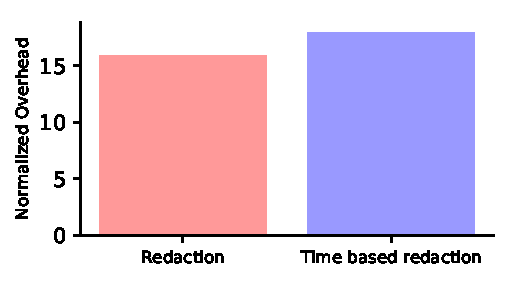
\includegraphics[width=8cm,height=4cm]{fig/policy_latencies.pdf}  
%%   \caption{Normalized latency of servicing an \texttt{open} for different policies with respect to the latency to service a null-policy capsule open request. }
%%   \label{fig:policy_latency}
%% \end{figure}
% %%%%%%%%%%%%%%%%%%%%%/


%% To identify the impact on applications operating on trusted capsules,
%% we look back and reference the work we had done for the first
%% generation prototype. Our experiences when creating the first
%% generation of the prototype have been our guiding principle for making
%% the system perform better. We present here the perceived latencies for
%% applications that operate on capsules while performing some
%% non-trivial tasks. \footnote{The reader is reminded that the following
%%   results are based on the first generation prototype which is based
%%   on the older system that used system call interceptor mechanism as
%%   described in ~\ref{sub:proto-prototype}}

%% We measured the impact under three different conditions: with an empty
%% null policy, with our use case policies, and without trusted capsules
%% (as a baseline). Some of our use case policies, such as those on the
%% PDF and JPEG, required a trusted capsule server in order to fetch
%% remote state and report logged information. For all data type
%% use-cases, we implemented use-case policies described in
%% Section~\ref{sec:new-policies}, except for redactions on PDF
%% documents, which required knowing PDF's binary format.

%% We used a Canon Rebel II DSLR to film certain interactions between the trusted capsule and applications. We then measured the latency between
%% the start of an action (e.g. open a document) and when the action is
%% completed. We filmed at 60 FPS and used the difference in timestamps
%% to calculate the application latency. We present our results in
%% Table~\ref{Tbl-Macro-performance} and provide the raw footage online:
%% \url{https://goo.gl/SiBEJB}.

%%%%%%%%%%



% We used Linaro OP-TEE OS (version 3.3) We modified the Linaro OP-TEE OS version
% 3.3 to be our TrustZone software stack and mounted a userspace filesystem in the
% normal world operating system that runs a custom Hikey Debian OS based on Linux
% kernel 4.4.15. \pu{check} In the FUSE filesystem, we intercept \textit{open} and
% \textit{close} system calls and redirect them to the secure world for decryption
% and encryption respectively. All accesses to non-capsule files proceed just like
% normal file operations on a FUSE mountpoint.

%We deployed ARM Trusted Firmware and a modified Linaro OP-TEE OS as our
%software stack in TrustZone.


%Our trusted capsule monitor in the normal world 
%consists of a modified Linaro OP-TEE supplicant and a modified Linaro OP-TEE Linux 
%Driver with our custom system call interceptor. The kernel components are deployed as
%Linux kernel module. 

% Our modifications to the OP-TEE OS in the secure world is limited to the
% implementation of a few missing \texttt{libc} functions like \texttt{atoi} and
% \texttt{strcmp}. These are minimal changes compared to the original OP-TEE code
% base.

%Our modifications to the OP-TEE components across the
%software stack in both worlds consist entirely of additional RPCs that 
%enable trusted capsule applications to access the file system and network
%directly. These modifications are minimal compared to the original OP-TEE
%code base. % Our implementation is based on OP-TEE 1.0. 


% twithin the OP-TEE Linux Driver that returns predefined longitude and latitude
% values.
%
% In the normal world, we run a pre-alpha release of a custom HiKey Debian OS
% based on Linux kernel 3.18.0.
%
% We used 128-bit AES and SHA-256 for encrypting and hashing trusted
% capsules.

% Our current implementation supports the following composable actions
% based on policy evaluation:

% \begin{itemize}

% \item Allowing or denying the operation on the trusted capsule.

% \item Initializing or modifying persistent state (e.g., counter).

% \item Performing byte-based or keyword-based redaction that partially
%   discloses trusted capsule data. %A data-type specific pre-processor
%   %can be used to generate the byte offsets.

% \item Reporting the operation, location, time, role-identity of the
%   device to a global policy coordinator.

% \item Hard access revocation by deleting the capsule, triggered
%   locally or remotely; and, soft revocation by arbitrarily changing
%   the policy.

% \item Prevent declassification through the network or file system.
% \pu{Review.}


%\item Registering a callback -- to place a deterministic real-time bound on when a policy is re-evaluated 
%\item Killing a running process 

%\end{itemize}

% In total, our trusted capsule application has 4.2K lines of
% non-comment C code and our filesystem code has 2K lines of
% non-comment C code.

%\include{discussion}
%\include{conclusions}

%    3. Notes
%    4. Footnotes

%    5. Bibliography
\begin{singlespace}
\raggedright
\bibliographystyle{abbrvnat}
\bibliography{biblio}
\end{singlespace}

\appendix
%    6. Appendices (including copies of all required UBC Research
%       Ethics Board's Certificates of Approval)
%\include{reb-coa}	% pdfpages is useful here
\include{appendix}

\backmatter
%    7. Index
% See the makeindex package: the following page provides a quick overview
% <http://www.image.ufl.edu/help/latex/latex_indexes.shtml>


\end{document}
